\section{Introduction}
\label{sec:introduction}
Global climate models have become vital tools for
simulating the present and future climate and for predicting important
climate trends.  However, current global models are limited in their
ability to represent many multi-scale aspects of atmospheric flows.
Their resolutions, limited by computational costs, are too coarse to
accurately represent key processes that span a wide range of temporal
and spatial scales.  High-resolution simulations are essential for
capturing these scale interactions and for accurately representing local
and regional phenomena such as convection, orographically induced
precipitation, mesoscale storm systems, and tropical cyclones.  Such
events have large regional impacts as well as broader feedbacks onto the
large-scale climate system.  Today, high-resolution General Circulation
Models (GCMs) used for global climate simulations can utilize uniform
grid spacings down to 10 km as documented by, e.g.,
\cite{manganello:12} or
\cite{kinter:13}.  However, they are computationally very expensive and
still unable to represent key processes such as clouds explicitly.
Exceptions are the cloud-permitting, partly cloud-resolving, global
simulations by
\cite{miura:07},
\cite{putman:11} or
\cite{miyamoto:13} that were run for short, multi-day time periods with
grid spacings in the 0.9--3.5 kilometer range.  To employ such high
resolutions over longer climate time periods, modelers typically use
limited-area models (LAMs) that focus the computational resources in
areas of interest.  A major drawback is that LAMs require their lateral
boundaries to be externally forced.  These boundary conditions are
typically derived from much coarser GCMs which use different numerical
schemes and physical parameterizations, thereby introducing possible
biases or numerical discrepancies.  In addition, it is an open question
how well LAMs can capture teleconnections of global large-scale dynamics
and localized features particularly for tropical cyclones and other
phenomena that have feedbacks onto the larger climate system.

Variable-resolution GCMs can utilize static or dynamic grid
refinements which are promising options to bridge the gap between global
and regional climate modeling.  Application examples for static (non-moving)
mesh adaptations are provided in, for example,
\cite{zarzycki2014using}, \cite{rauscher2014impact}, \cite{zarzycki2015tropical} and
\cite{huang:16} (see also further references therein).  This chapter
focuses on dynamically adaptive grids, which track features of interest
during the model simulation by locally adding or removing grid points as
needed.  Adaptation criteria based on error estimates (e.g.
\cite{skamarock1989adaptive},
\cite{behrens1998atmospheric}, and
\cite{blaise2012dynamic}) or flow characteristics (e.g.
\cite{hubbard2003three}, 
\cite{jablonowski2006AMR,jablonowski2009AMR} and
\cite{st2007comparison}) can be used to determine
where the high-resolution mesh should be placed.  By increasing
resolution only locally, dynamic refinement significantly decreases the
total number of degrees of freedom for the simulation.  However, since
dynamic refinement is used within a global model, it also eliminates the
need for forced boundary conditions and solves the local high-resolution
area and global flow using the same dynamical core and physics package.
Global models allow for a better representation of global and
synoptic-scale phenomena and permit them to interact better with meso-
and small-scale features that can be resolved in the model.
Additionally, a key advantage of dynamic refinement compared to a static
refinement setup is that the location of the refined area does not have
to be determined \emph{a priori}.  

Adaptive refinement methods are
well established in many areas of computational fluid dynamics like aerospace engineering or 
space weather modeling (see e.g. \cite{toth2012adaptive}). In atmospheric science though, the
costs and benefits of AMR methods have mostly been
evaluated in idealized simulations and simplified models so far.  
Some of the first adaptive atmospheric models were developed by
\cite{skamarock1989adaptive},
\cite{skamarock1993adaptive}, and
\cite{Dietachmayer:1992sj}.  In general, the grid refinement strategies can be
categorized into three overarching types:  \emph{r}-refinement (or \emph{r}-adaptivity),
\emph{h}-refinement, and \emph{p}-refinement.

In \emph{r}-refinement, the number of grid cells remains unchanged;
instead, the cells are dynamically redistributed to increase resolution
in parts of the grid while decreasing it everywhere else.  This dynamic
grid adaptation creates smoother transition regions between resolutions but
requires a complex global remapping of the mesh to move the location of
the high resolution.
\cite{Dietachmayer:1992sj} uses this global grid redistribution
technique to increase resolution in areas where the estimated solution
error is high.
\cite{giraldo2000lagrange} and
\cite{iselin2002dynamic} have also applied this type of dynamic
adaptation for the 2D shallow-water equations and advection problems,
respectively.  More recently,
\cite{kuhnlein2012modelling} implemented \emph{r}-adaptivity within a 3D
Cartesian framework,
\cite{bauer2014simulation} used \emph{r}-refinement grids guided by
error estimates in a shallow-water model, and
\cite{weller2016mesh} demonstrated \emph{r}-refinement use on the
sphere.

Adaptive mesh refinement (AMR),
another term for \emph{h}-refinement,
increases resolution locally either by adding cells within the grid
structure or by overlaying additional cells of finer resolution on top
of the grid without changing the base grid structure.
\cite{skamarock1989adaptive} and
\cite{skamarock1993adaptive} implemented AMR by placing finer-resolution
meshes over the coarse grid in areas which had large truncation error
estimates.  The grid-cell solutions and boundary conditions between the
higher-resolution meshes and the base grid are continually updated.  In
a more recent example,
\cite{Chen:2011kk} use AMR that overlays high-resolution meshes in areas
of interest in a shallow-water model on a cubed-sphere grid.
Examples of AMR techniques that locally add and remove cells to the base
grid for the shallow-water equations on the sphere have been presented
by
\cite{behrens2005amatos},
\cite{lauter2007parallel},
\cite{st2007comparison} and
\cite{marras2015simulation}.  Both
\cite{behrens2005amatos} and
\cite{lauter2007parallel} use conformal unstructured finite element
meshes.  In conformal grids, each cell shares an edge with exactly one
other cell, while on a nonconforming grid, cells can share an edge with
more than one neighboring element.  The two AMR models described in
\cite{st2007comparison}, a block-structured finite-volume method on a
latitude-longitude grid and a spectral-element method on a cubed-sphere
grid, use nonconforming meshes and a quad-tree based AMR method with
gradient- or vorticity-based refinement criteria.
\cite{marras2015simulation} compared the use of an AMR approach on
several structured and unstructured non-conformal grids.  Use of AMR in a
regional model paired with a physical parameterization package was
presented in \cite{bacon2000dynamically}.
Furthermore, AMR methods have also been investigated for 
2D flow fields in Cartesian geometry. Recent examples include 
\cite{muller2013comparison} and \cite{kopera2014analysis} 
who analyzed a tree-structured AMR algorithm for 
non-hydrostatic dynamical cores in the x-z plane, and  
\cite{hendricks2016evaluation} who explored static and dynamic AMR for 
tropical-cyclone-like vortices in a shallow-water model 
on an $f$-plane with a constant Coriolis parameter $f$.

The third type of dynamic refinement, \emph{p}-refinement, holds the
grid spacing fixed but changes the order of the polynomial approximation
within each grid element to increase local resolution.  Use of \emph{p}-refinement
with Discontinuous Galerkin (DG) methods for the shallow-water equations
were described by \cite{kubatko2009dynamic} and
\cite{tumolo2015semi}.  A hybrid refinement method that combines the
\emph{h}- and \emph{p}-refinements methods was demonstrated by
\cite{eskilsson2011hp}, and
\cite{blaise2012dynamic} used an \emph{hp}-adaptive DG method to model
the shallow-water equations on the sphere for global tsunami
simulations.  Recently,
\cite{aechtner2015conservative} implemented a new adaptive wavelet
approach for local dynamic refinement with the 2D shallow-water
equations on the sphere.

The purpose of this study is to demonstrate the pros and cons of using
AMR, \emph{h}-refinement, for simulating atmospheric flows.
It assesses the effectiveness of AMR, employing a 
non-conformal grid, in achieving
similar results as uniform-grid simulations while reducing computational cost. Furthermore,
it is revealed that AMR can be implemented without harming or degrading the
large-scale smooth flows or inducing numerical noise and wave-like
reflections at AMR boundaries.  The 2D shallow-water equations serve as
a useful testbed for an AMR model as they exhibit many of the
complexities present in a full 3D model.  We utilize the cubed-sphere
fourth-order finite-volume AMR model presented in
\cite{mccorquodale2015adaptive} for the 2D shallow-water equations on
the sphere.  The model implements a mapped-multiblock AMR technique that
overlays refined patches on the coarser grid. Our work tests
the model's ability to track and refine over dynamic small-scale
features of interest and to evaluate refinement criteria.  We
investigate various refinement criteria, such as thresholds for the
height gradient or relative vorticity, that guide the locations of refinement
patches.  In addition, we shed light on factors that may limit AMR
applications including the size of the refinement ratios between grid
levels and the total number of levels.  Lastly, we examine the
effect of AMR on large relatively smooth flows where extra refinement is
unnecessary.  Specifically we focus on how the coarse-fine interfaces of
the AMR patches influence the overall flow and error.

The chapter is organized into three main sections.  A brief
description of the model and a discussion of the multiblock AMR
techniques are provided in Section~\ref{sec:model}.
Section~\ref{sec:results} discusses the results of the numerical tests.  One advection test and four
shallow-water tests are presented.  The tests are the moving vortices
advection test by \cite{Nair:2008fk}, a steady-state geostrophic flow
(test case 2 from \cite{Williamson:1992kx}), the unsteady solid body rotation test of
\cite{Lauter:2005uq}, a shallow-water test consisting of a gravity wave
impinging on an isolated mountain, and lastly a test that assesses the
interaction of idealized binary vortices.  Conclusions are provided in
Section~\ref{sec:conclusion}.

\section{Model Description}
\label{sec:model}

The Chombo-AMR dynamical core (dycore) is a new model that is built upon
an unstaggered high-order finite-volume (FV) multiblock approach with a
classical fourth-order Runge-Kutta (RK4) time discretization scheme. 
A detailed description of the model
setup to solve the shallow-water 
equations in conservative flux form can be found in
\cite{mccorquodale2015adaptive}.  In addition, the Chombo AMR library is
described in
\cite{Adams:2015gd}.  

The shallow water equations on the sphere in coordinate invariant form
are given by
\begin{equation}
   \label{eq:swmom} \frac{\partial h \mathbf{v}}{\partial t} +
     \nabla \cdot \left( h \mathbf{v} \mathbf{v} + \mathcal{I} \frac{g h^2}{2} \right) =
      - g h \nabla z_{\rm s} - f \mathbf{k} \times (h \mathbf{v})
\end{equation}
\begin{equation}
     \label{eq:swcon}  \frac{\partial H}{\partial t}+ \nabla \cdot (h \mathbf{v}) = 0
\end{equation}
where $\mathbf{v}$ is the velocity vector, $\mathbf{v}\mathbf{v}$ 
denotes the outer product of the velocity vector, 
$\mathcal{I}$ is the identity matrix, $f = 2 \Omega \sin \phi$
is the Coriolis parameter in terms of the angular rotation 
$\Omega = 7.292 \times 10^{-5}\ \mbox{s$^{-1}$}$, and 
$g = 9.80616\ \mbox{m}\ \mbox{s}^{-2}$ is the acceleration due to 
gravity. $H$ denotes the total height of the fluid surface. Bottom topography $z_s$
and $h$, the fluid depth above bottom topography, relates to the total height
by $H = h +z_s$.

The finite-volume approach is implemented on an
equiangular cubed-sphere grid.  This grid consists of six separate
panels that are projected onto the surface of the sphere.  The mesh thereby
eliminates the singularities due to converging meridians at the
poles found in spherical latitude-longitude grids.  Additionally, the
equiangular cubed-sphere leads to a quasi-uniform spherical grid with
grid cells of similar size across the sphere.  The discrete resolution
of the cubed-sphere grid is represented as $c\{N_c\}$ where $N_c$
denotes the number of grid cells in each direction on the six panels.  A
list of properties of the equiangular cubed-sphere grid, including the
approximate grid spacings, is given in
Table~\ref{tb:grids} for several resolutions.  The finite-volume method for
the spatial discretization uses a fourth-order accurate discretization
to compute flux averages on the faces.  The central difference operators
used to obtain the fluxes are smoothed by an explicitly added sixth-order diffusive
operator which maintains the fourth-order accuracy of the scheme
 (see \cite{mccorquodale2015adaptive} for details).
No additional limiters or filters are
implemented.  The numerical scheme is 
mass-conserving to machine precision and energy-conserving up to the
temporal truncation order, when used without limiters or explicit
dissipation.  The total-energy conservation properties for the model
with added dissipation are demonstrated in Fig.~11 of
\cite{mccorquodale2015adaptive}.

\begin{table}[t]
    \caption{Properties for several cubed-sphere grid resolutions where 
    $N_c$ is the number of cells along an edge of a cubed-sphere panel.
    Here the number of cells is the total number of grid cells 
    ($N_c^2 \times 6$), $\Delta x$ is the approximate grid spacing, 
    $A_{avg}$ is the average area of a grid cell, $A_{min}/A_{max}$ is the
    ratio between the minimum and maximum cell areas, Eq.  Res.  is the
    grid resolution in degrees given by $90^\circ / N_c$, and $RLL_{equiv}$
    is the equivalent grid spacing on a regular latitude-longitude
    grid with the same total number of cells.}%
    \label{tb:grids}
    \begin{center}
        \resizebox{\textwidth}{!}{
    \begin{tabular}{cccrccc}
            \hline
            Resolution ($N_c$) & No. of cells       & $\Delta x$ (km) & $A_{avg} (\mbox{ km}^2)$ & $A_{min}/A_{max}$ & Eq. Res.     & $RLL_{equiv}$ \\ 
            \hline
            \hline
            c$16$              & $1.54 \times 10^3$ & $625$           & $3.321 \times 10^{5}$    & $0.7434$          & $5.63^\circ$ & $6.50^\circ$  \\ 
            c$32$              & $6.14 \times 10^3$ & $313$           & $8.302 \times 10^{4}$    & $0.7249$          & $2.81^\circ$ & $3.25^\circ$  \\ 
            c$64$              & $2.46 \times 10^4$ & $156$           & $2.076 \times 10^{4}$    & $0.7159$          & $1.41^\circ$ & $1.62^\circ$  \\ 
            c$128$             & $9.83 \times 10^4$ & $78.2$          & $5.189 \times 10^{3}$    & $0.7115$          & $0.70^\circ$ & $0.82^\circ$  \\ 
            c$256$             & $3.93 \times 10^5$ & $39.1$          & $1.297 \times 10^{3}$    & $0.7093$          & $0.35^\circ$ & $0.41^\circ$  \\ 
            c$512$             & $1.57 \times 10^6$ & $19.5$          & $3.243 \times 10^{2}$    & $0.7082$          & $0.18^\circ$ & $0.20^\circ$  \\ 
            c$1024$            & $6.29 \times 10^6$ & $9.77$          & $8.107 \times 10^{1}$    & $0.7076$          & $0.09^\circ$ & $0.10^\circ$  \\ 
            \hline
        \end{tabular}
        }
    \end{center}
\end{table}

Since high-order FV schemes make use of neighboring elements, 
a mapped-multiblock approach is used to coordinate the remapping of
element 
values that are needed for the flux calculations across panel boundaries on the
cubed-sphere.  Though the cells at panel edges are conformal with
neighboring cells across panel boundaries, the transition between the
panels is not smooth due to the separate mapping on each panel.  To
preserve the order of accuracy of the fluxes, the domain is expanded at
the panel edges with the addition of three layers of ghost cells to perform the FV
calculations on each panel.  As a result of different mappings, ghost
cells of one panel will not have the same shape as cells on the
neighboring panel.  Therefore, the values in the ghost cells are set by
least-squares interpolation from a stencil of surrounding cells that are
within the domain of the ghost cell's panel and on neighboring panels 
(Sec. 3.4 in \cite{mccorquodale2015adaptive}
 describes in detail the interpolation process).
Additionally, flux values for the cell faces that lie on a panel edge
are calculated separately for each panel, and the mean of the 
two fluxes is taken as the value  
for that face to ensure conservation. 
Thus communication between the separate domains
for each panel is limited to the fluxes at the domain boundary and the
neighboring cell values needed to interpolate the solution to the ghost
cell regions.  The block-structured AMR method allows for further
subdivision of the computational domain of each panel into rectangular
regions of grid cells called patches, which allow the calculation to be
distributed efficiently on parallel computing platforms.

\subsection{Adaptive Mesh Refinement}
\label{subsec:AMR}

Our 2D AMR shallow-water model
uses the strategies within the Chombo library \citep{Adams:2015gd} that
has been designed for parallel computing architectures.  AMR
calculations are performed on a hierarchy of nested meshes, called
levels, which have a defined refinement ratio between them. This refinement ratio must be a power of two. The finer
levels are overlaid on top of the coarser levels and are organized in
the block-structure described in the previous section.  
Figure~\ref{fig:cyclesnlevels}a provides an example of the AMR grid structure with two refinement levels.
Whenever new cells are created, they are initialized via interpolations from the coarser level and ghost cells
are used to calculated the fluxes at patch boundaries.  At these
coarse-fine interfaces, as at panel boundaries, the space-time accuracy
drops from fourth-order to third-order due to a lack of error
cancellation that would normally occur with the FV method.  Intermediate
levels must have a sufficient number of cells separating a finer level
and a coarser one. This ensures that the finer level is properly nested so that
the interpolation to fill ghost cells on the finer-level can be
performed using cells from only one level.

\begin{figure}
    \centerline{%
    \noindent
    \includegraphics[width=\textwidth]{Chap1/subcyles_and_levels_h.eps}}
    \caption{(a) Example of a grid with two levels of AMR using a x2
    refinement ratio between levels.  The additional levels do not
    replace the coarse level cells underneath, they are overlaid on top.
    (b) Diagram depicting the sub-cycling of AMR levels in time.  The
    coarse level is advanced first from time $t_n$ to time $t_n +\Delta t$ where $\Delta t$ is the time step for the coarsest level. Then the finer levels are advanced
    with a smaller time step and periodic updates of fluxes from the
    coarser grids.}%
    \label{fig:cyclesnlevels}
\end{figure}

Figure~\ref{fig:cyclesnlevels}b depicts an overview of the time-stepping and 
sub-cycling process. Rather than having a uniform
time step dependent on the smallest grid-cell size, Chombo-AMR
sub-cycles the refined levels in time maintaining a constant Courant
number.  As noted by \cite{ullrich2014understand} the single-wave-mode characteristics of a numerical method often have an
unexpected and non-linear dependence on the Courant number.
Therefore, a constant Courant number helps ensure consistent dispersive
properties across the refinement levels. 
The typical work flow for advancing an AMR grid level $l$ in time is as
follows:
\begin{itemize}
    \item[1.]
        Regrid levels finer than $l$ if required:  \newline Evaluate the refinement criterion
        and mark (tag) all cells which should be included in finer levels.
        In these regions, new blocks of cells at levels $l+1$ are
        overlaid.  The new cell values are interpolated from the coarser
        level using a fourth-order least-squares algorithm that maintains
        conservation as described in Sec. 4.1 of \cite{mccorquodale2015adaptive}.
    \item[2.]
        Advance level $l$ one time step using the RK4 time-stepping
        method.
    \item[3.]
        Interpolate values to the ghost cells that surround level $l+1$
        using the least-squares algorithm also implemented for ghost cells 
        at panel boundaries. Three layers of ghost cells
        are required.  The interpolation does not need to be
        conservative as the ghost cell values are only used to
        reconstruct the flux on the faces of the level $l+1$ cells.
        Figure~\ref{fig:ghost_cells} depicts the location of ghost cells for 
        two of the three layers and the stencil of coarse grid cells used 
        for their interpolation.
    \item[4.]
        Perform previous steps for level $l+1$.  Level $l+1$ is
        advanced using refined time steps (sub-cycling) as depicted in
        Fig.~\ref{fig:cyclesnlevels}b.  A temporal interpolation closely
        related to the RK4 method is used to update the values in the 
        level $l+1$ ghost cells from cells on level $l$ at the intermediate time
        steps \citep{mccorquodale2015adaptive}.
    \item[5.]
        After the sub-cycling in time is completed, average the solution
        from level $l+1$ and sum up the fluxes to update the values on
        the coarse grid.  Corrections are applied to the fluxes at
        coarse-fine interfaces to ensure conservation \citep{berger1989local}.
\end{itemize}

\begin{figure}
    \centerline{%
    \noindent
    \includegraphics[width=19pc]{Chap1/cs_amr_ghostcell.png}}
    \caption{Example of a 1-level AMR approach with a refinement ratio of two
    on the cubed sphere grid.  The four dashed cells are schematic examples of ghost
    cells for the finer grid, which are interpolated from the values in
    the coarse cells shaded in gray. Our actual AMR applications need three ghost cells.}%
    \label{fig:ghost_cells}
\end{figure}

As mentioned in the description of the first step, the additional levels are placed in
locations that have been tagged by the refinement criterion of the
model.  The size of the refined grid that is added over tagged cells is
determined by three aspects: (1) the need to ensure proper nesting of finer levels,
(2) parameters from the Chombo library designed for efficient
parallelization, and (3) a user-defined buffer parameter.  Refinement (tagging)
criteria are based on thresholds for user-selected flow properties, like
relative vorticity, that indicate where refinement should be placed.
The tagging strategies can be based on a variety of properties including
tracer values, vorticity thresholds, gradients, or a combination of
several criteria.  The type of refinement criteria and the threshold
values are set independently for each simulation.  The threshold values
can be uniform across all refinement levels or designed to scale with
increasing refinement.  For example, the relative vorticity threshold can be set
so that it increases with increasing resolution. With the idealized
test cases presented in this chapter, the selection of refinement criteria
and thresholds was problem-dependent, with the simplicity of the
tests offering only a few possible options.  A range of refinement
thresholds for the AMR test cases was explored. Here, we present 
various thresholds for the gravity wave and binary vortices tests to
demonstrate how changes in refinement affect the solutions and grids.
For the moving-vortices advection test we only present a single 
threshold value that represents a compromise between reducing the
error and increasing the computational run time.

The Chombo-AMR dycore is designed to have multiple refinement levels (up
to ten), and the maximum number of levels is set for each simulation.
In our simulations, we explore the effects of adding up to
two refinement levels (called 2-level AMR).  In addition, we explore the
grid-resolution refinement ratios between successive levels,
and present selected results for three powers of two: x2, x4 and x8.
As an example, a grid with a base level of
c32 ($2.8^\circ$) resolution and 2 levels of x4 refinement has
a maximum resolution of c512 ($0.18^\circ$). 

\section{Results of the Numerical Experiments}
\label{sec:results}
For our assessment of the
Chombo-AMR shallow-water model, we select five test cases: one advection
test and four shallow-water tests.  The test cases are divided into two
categories:  large-scale smooth flows and
simulations with either sharp gradients or strong, non-linear, localized
flows.  The first category is comprised of the following two
shallow-water tests:
\begin{itemize}
    \item
        a steady-state geostrophic flow (test case 2 in
        \cite{Williamson:1992kx})
    \item
        an unsteady solid body rotation (example 3 from
        \cite{Lauter:2005uq}).
\end{itemize}
These large-scale flows, which have no realistic use for AMR, serve as
``do no harm'' tests.  They are used to check the model's ability to
preserve the characteristics of smooth flows as they cross the AMR
patches.  We measure the impact that the refinement ratios, the number
of AMR levels, and the location of the refinement patches have on the
solution.  Convergence tests are also performed with these test cases that both have analytical solutions.

The second test category with localized flow features consists of three tests for which
AMR could improve the solution, and we seek to evaluate how effectively
it is able to do so. These tests are
\begin{itemize}
    \item
        the moving vortices advection test by
        \cite{Nair:2008fk} (with analytical solution)
    \item
        a gravity wave impinging on an idealized mountain shallow-water
        test.
    \item
        a binary-vortices test case in which two vortices interact.
\end{itemize}
The bottom two do not have analytical solutions and the evaluations rely on
high-resolution reference solutions.
A variety of refinement criteria are used with these test cases to
demonstrate the AMR's ability to track, adapt to, and resolve these
localized features accurately.  The model results are presented using
normalized $l_2$ and $l_\infty$ error norms as defined in
\cite{Williamson:1992kx}.  Additionally, the total number of grid cells
quoted for AMR runs include the sum of all valid grid cells from all
refinement levels (not including ghost cells) since the finer levels
overlay the coarser grids beneath them.  The total number of grid cells
can serve as a rough benchmark of computational cost when comparing AMR
runs to uniform runs.

The model results are presented using
normalized $l_2$ and $l_\infty$ error norms as defined in
\cite{Williamson:1992kx}. These errors for computed variable field $h$ are calculated
 via the usual global error norms,
\begin{equation}
   \label{eq:l2} l_2(h) = \sqrt{\frac{I\left[(h-h_\tau)^2\right]}{I\left[h_\tau^2\right]}}
\end{equation}
\begin{equation}
   \label{eq:lmax} l_\infty(h) = \frac{\max|h-h_\tau|}{\max|h_\tau|}
\end{equation}
where $h_\tau$ is the reference field and $I$ is a discrete approximation
to the global integral given by
\begin{equation}
    \label{eq:globint} I[x] = \sum_{\text{all cells } k} x_k A_k
\end{equation}
where $A_k$ denotes the area of grid cell $k$.

\subsection{Moving-Vortices Advection Test} 
\label{subsec:moving-vortices}

The moving-vortices test is
a challenging deformational-flow advection test proposed by
\cite{Nair:2008fk}.  The test represents the roll-up of an initially
smooth tracer into tight spiral bands. The roll-up creates steep
gradients which provide a good test for the AMR.  In this test, a pair
of vortices is generated on diametrically opposite sides of the sphere.
The wind field is the summation of a solid-body rotation and a
deformational flow such that the two vortices move along a great circle 
and an exact solution is known at all times [see \cite{Nair:2008fk} for details].

A 12-day time period is simulated,
which advects the spiraling vortices once around the sphere.  The
background flow is prescribed with a rotation angle of $\alpha=\pi/4$
so that the two vortices are advected through the corners of the
cubed-sphere (located at $\pm 45^\circ$).
Figures~\ref{fig:spradverrplots}a--d depict the analytical solution for the roll-up of the tracer at
days 0, 4, 8, and 12.
%
\begin{figure}
    \centerline{%
    \noindent
    \includegraphics[width=\textwidth]{Chap1/sprl_adv_err.eps}}
    \caption{(a)--(d): Analytic tracer field at days 0, 4, 8, and 12
for the moving-vortices advection test of
Section~\ref{subsec:moving-vortices}.
    (e)--(h): Tracer error at the select days for a 2-level AMR run with a
    c32 base resolution using x4 refinement (c32/c128/c512) and the
    tracer-gradient refinement tagging criterion.  (i)--(l): same as (e)--(h)
    but with the combination of relative-vorticity magnitude and tracer-gradient
    criterion.  The adaptive block-structure is shown by black
    lines.  The thickest lines are the base c32 grid, and thinner lines
    represent the c128 and c512 levels.  Note (e)--(h) have different
    contour scale than (i)--(l).}%
    \label{fig:spradverrplots}
\end{figure}
%
Numerical tests were carried out with uniform grids and AMR grids with
two different tagging criteria:  a tracer-gradient tagging and a
combination tagging.  In tracer-gradient tagging, the model refines in
regions where $|\nabla q| > 1.5 \times 10^{-7}$ $\mathrm{m}^{-1}$,
where 
$q$ is the unitless value of the passive tracer.  Combination tagging
combines the tracer-gradient tagging criterion with a relative-vorticity
tagging that refines in areas where 
$| \zeta | > 1.45 \times 10^{-5}\mathrm { s}^{-1}$, 
so that the model refines over regions in which either
threshold is reached. 
The gradient threshold value demonstrates a balance between 
reducing error and limiting computational costs. 
A lower threshold increases run time without significantly 
reducing error and a higher one results in a large increase in error. 
The vorticity threshold is set to maximize initial refinement around 
the vorticity patches without being 
too low as to refine on the background vorticity.
With both criteria, a x4 refinement ratio between
levels was used.  The evolution of the grids can be seen in
Fig.~\ref{fig:spradverrplots}, which shows the tracer error for the two AMR
runs. 
Figures~\ref{fig:spradverrplots}e--h depict the 2-level AMR run (c32/c128/c512),
which has a base grid with c32 resolution, a c128 intermediate AMR
level, and a finest c512 AMR level, using the tracer-gradient tagging.
Figures~\ref{fig:spradverrplots}i--l depict the same 2-level AMR setup but with
the combination tagging.  The adaptive block-structure is clearly
successful at tracking the evolving vortices.  The block structure of
patches, not the individual grids cells, is outlined by the black lines
in Fig.~\ref{fig:spradverrplots}.  Each patch contains a user-selected maximum
number of grid cells.  However, patches might also be split into smaller
blocks by the Chombo library.  This optimizes the load-balancing of the
model on parallel computing architectures and increases the efficiency of
the code.  Therefore, various patch sizes are present in
Fig.~\ref{fig:spradverrplots}.
%
\begin{figure}
    \centerline{%
    \noindent
    \includegraphics[width=\textwidth]{Chap1/final_sprl_adv_err_grid_plots_w16.eps}}
    \caption{
For the moving-vortices advection test of
Section~\ref{subsec:moving-vortices},
growth over time of:
(a) normalized $l_2$ tracer error, and (b)
    total number of grid cells.  The plots
    provide a comparison of uniform runs (solid lines, no markers) and
    AMR runs using gradient tagging (broken lines, with and without
    markers) and combination of relative-vorticity and tracer-gradient
    tagging (solid lines with markers).  All AMR runs use the x4
    refinement ratio between resolution levels.}%
    \label{fig:spradvl2err}
\end{figure}
%
For the tracer-gradient tagging scheme
(Figs.~\ref{fig:spradverrplots}e--h), the error is largest near the center of
the spiral. The combination tagging scheme
(Figs.~\ref{fig:spradverrplots}i--l) significantly reduces the error near the
center, and the largest error is now towards the outer edges of the
spiral just beyond the coarse-fine grid boundaries.  When using only the
tracer-gradient tagging, refinement does not begin until after day one,
so errors accumulate on the coarse grid until that time and remain
higher even after being overlaid with finer levels.  With the
combination tagging, the central region is already refined (see
Fig.~\ref{fig:spradverrplots}i), which limits the error growth.  This effect
can also be seen in
Fig.~\ref{fig:spradvl2err}a where a time series of the normalized $l_2$
tracer errors with respect to the analytic solution are depicted for 15
different model configurations.  In particular,
Fig.~\ref{fig:spradvl2err}a compares the $l_2$ tracer errors of the five
uniform-resolution simulations c32, c64, c128, c256, and c512 (see
Table~\ref{tb:grids} for the associated grid spacings) to various 1-level and
2-level AMR experiments with either the tracer-gradient or combination
tagging.  The time evolution of the associated total number of grid
cells, including the underlying coarse cells, is shown in
Fig.~\ref{fig:spradvl2err}b.  In general, the error in the combination
tagging simulations reaches the lower error values of the uniform runs
(with the same resolution as the finest AMR level) more quickly than the
tracer-gradient tagging ones, despite having a significant
difference in grid-cell count for only the first few days (see
Fig.~\ref{fig:spradvl2err}b).
The errors in all
single-level AMR runs in
Fig.~\ref{fig:spradvl2err}a using both tagging criteria converge to the error
of uniform runs at the highest resolution (e.g., the c32/c128 AMR run and
the uniform c128 run).  This result is achieved using significantly
fewer grid cells than the uniform runs.  AMR limits the normalized 
$l_2$ error growth.  AMR runs begin with global errors that are near the level 
of uniform runs with a grid resolution of their coarsest grid.
However, their global error increases at a much slower rate than that of
the uniform runs until the AMR error approaches the error level of the
matching high-resolution uniform run.  In the simulations presented here the 2-level AMR runs see a diminishing
effectiveness at decreasing the global error as the errors from the
coarse section of the grid dominate. 
%
\begin{figure}
    \centerline{%
    \noindent
    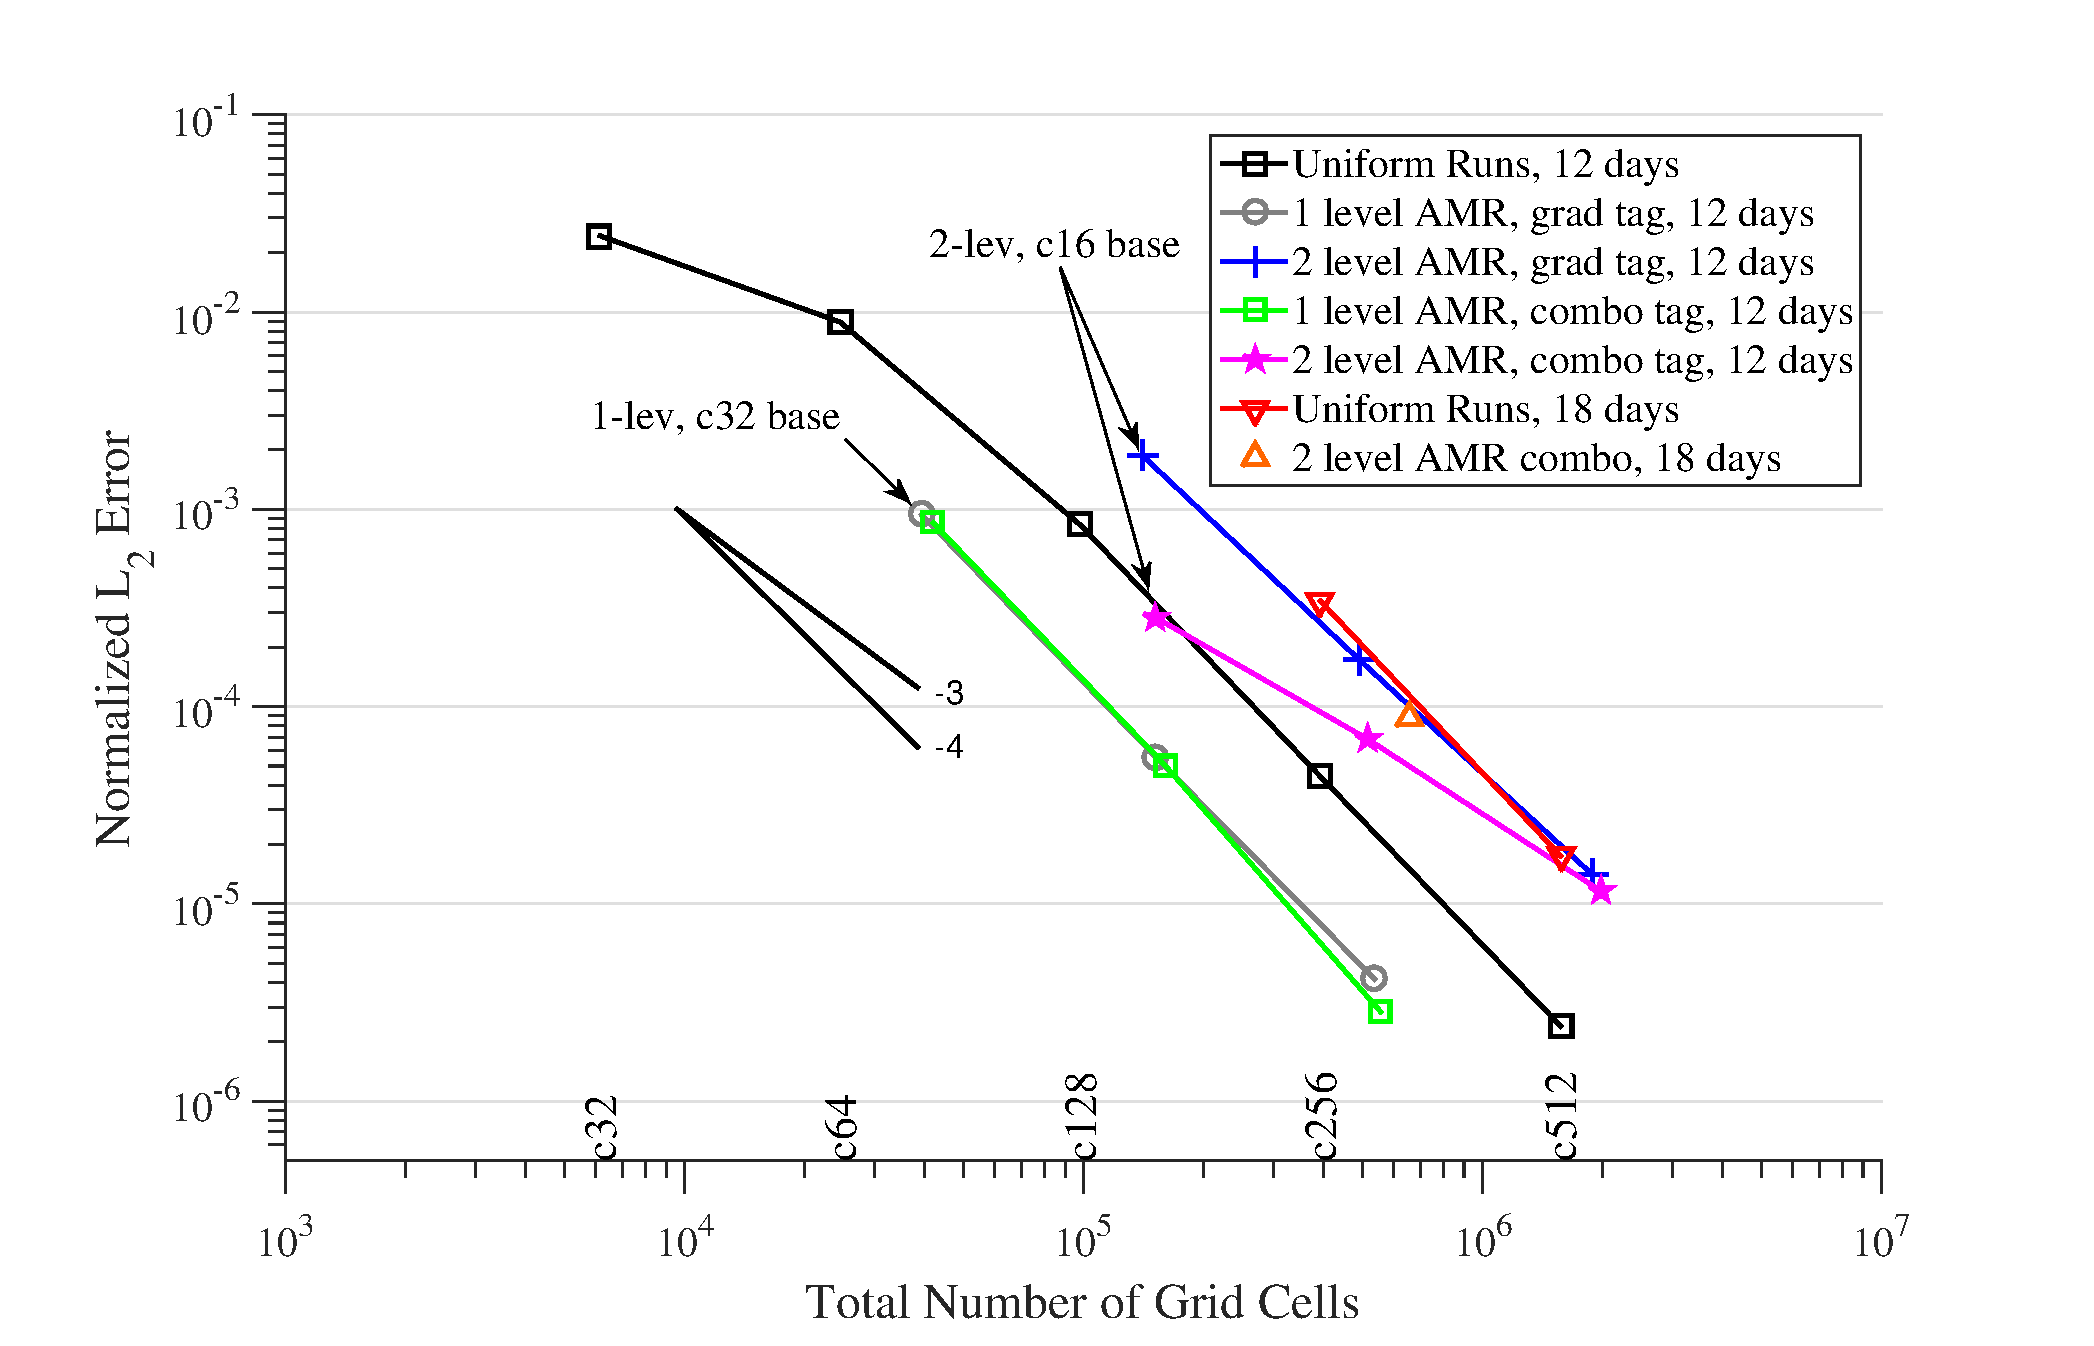
\includegraphics[width=\textwidth]{Chap1/sprladv_errvsgrid.eps}}
    \caption{Normalized $l_2$ gradient error as a function of total
    number of grid cells for the moving-vortices advection test case of
Section~\ref{subsec:moving-vortices}
 at day 12.
    The grid-resolution labels along the bottom axis note the number of
    grid cells in the uniform grids with those resolutions.  The black
    square markers are for the uniform runs c32 through c512.  The gray
    circles and green squares represent the 1-level x4 refinement AMR
    with base resolutions of c32, c64, and c128 using gradient tagging
    and combination tagging, respectively.  The blue crosses and magenta
    stars represent the 2-level x4 refinement runs with base
    resolutions of c16, c32, and c64 using gradient tagging and
    combination tagging, respectively.  Finally, the red downward-pointing
    triangles represent the uniform c256 and c512 runs at day 18, while
    the orange triangle is the 2-level x4 refinement runs with a c32
    base resolution, using the combination tagging at day 18.  Solid
    black lines depict convergence rates.}%
    \label{fig:spradvl2vgrid}
\end{figure}
%
The error at day 12 as a function of total number of grid cells for both
uniform and AMR runs is plotted in
Fig.~\ref{fig:spradvl2vgrid}.  AMR runs that have error values plotted to the
left of the errors of the uniform runs (line of hollow black squares)
achieve a lower $l_2$ error than a uniform run with a comparable
number of grid cells.  While the 1-level AMR runs show a decrease in
error while using fewer grid cells, the 2-level AMR runs generally result in a
higher error for a comparable number of grid cells than the uniform runs.  Only
the 2-level AMR run with a c16 base using the combination tagging has a
slightly improved error compared to the uniform runs (see the leftmost magenta star).  
These results demonstrate the reduced improvement to the global error from additional
levels of AMR with very coarse base meshes.  
However, AMR still slows down the error growth over time in comparison to uniform runs, and even asymptotes
to the finest uniform mesh errors (c128/c512, for example).  
Extending the run
time to 18 days, the $l_2$ error from the c32 base 2-level AMR run
with the combination tagging (orange triangle in
Fig.~\ref{fig:spradvl2vgrid}) is now slightly lower than the error from the
uniform runs at day 18 (red downward-pointing triangles).
Figure~\ref{fig:spradvl2vgrid} also confirms that the convergence rate for the
uniform run is fourth-order in the normalized $l_2$ error.

\cite{Nair:2008fk} applied this test using an $\alpha=0^\circ$ setup (not
$\alpha = 45^\circ$ as we present here) in an FV-AMR model 
using a coarse $5^\circ$ base grid and one to three levels of x2
refinement which were guided by a tracer-gradient threshold.  Their AMR errors
were generally the same or lower than the errors of their comparable uniform
runs for coarse grids with one or two levels of refinement.  However,
for their 3-level AMR run (finest resolution $0.625^\circ$) errors were
slightly higher than their uniform $0.625^\circ$ run, agreeing with what we observe for
multiple levels of AMR.  Additionally, our error measures for uniform-resolution runs are
comparable to other higher-order models.  Our uniform c64 
($\sim 1.4^\circ$) run with 
$\alpha=45^\circ$ has a normalized $l_2$ error of $8.9\times 10^{-3}$ 
after twelve days, which is comparable to the results from the 
$1.25^\circ$ grid using a multi-moment method in
\cite{chen2011multi} and slightly higher than the c80 ($1.125^\circ$) run
in
\cite{lauritzen2010conservative}.
%
\begin{table}
    \caption{Run times (wall-clock time in s and as \% of c512 run time)
for 12-day moving-vortices advection simulations
(Section~\ref{subsec:moving-vortices}).
    These runs had a maximum resolution of
    c512, performed on two nodes of NCAR's Yellowstone computing platform with 32 processors total. 
    Number of cells per refinement level is given at day 12, and
    as a percent of the c512 uniform run. }%
    \label{tb:adv_time}
    \resizebox{\textwidth}{!}{
    \begin{tabular}{rcrrrrrr}
        \hline
        Base Res.          & AMR Levels         & Run Time (s)            & Run Time (\%)            & c32 cells               & c128 cells              & c512 cells          & Total cells (\%) \\ 
        \hline
        \hline
        c512               & -                  & $24152$                 & $100\%$                  & $0$                     & $0$                     & $1.6 \times 10^{6}$ & $100\%$          \\ 
        c128               & 1                  & $10116$                 & $42\%$                   & $0$                     & $9.8 \times 10^{4}$     & $4.5 \times 10^{5}$ & $34\%$           \\ 
        c32                & 2                  & $10468$                 & $43\%$                   & $6.1 \times 10^{3}$     & $4.2 \times 10^{4}$     & $4.6 \times 10^{5}$ & $32\%$           \\ 
        \hline
        \hline
    \end{tabular}
    }
\end{table}
%
We also include the total run time versus number of grid cells in 
Table 
\ref{tb:adv_time},
for some of the 12-day runs  in
Fig.~\ref{fig:spradvl2vgrid}.
In this case, the wall-clock time (as a \% of the finest uniform run)
is closely related to the total number of grid points, because most of
the time steps and grid cells are at the finest level.
For AMR runs, coarser levels must be completed before fine levels.
There is therefore a slight performance penalty for the 2-level AMR (c32/c128/c512)
run, which actually increases the total number of finest-level points. This configuration
only has 24 boxes (each $16\times16$ cells) at the c32 level to be
distributed across 32 processors on the Yellowstone computing platform (operated 
by the National Center for Atmospheric Research (NCAR)). This means that some processors run idle when the
solution on the coarsest grid is computed which slightly lessens the parallel performance
of this AMR run.
Overall, a good heuristic for this test is that the run time is 
approximately proportional to the total number of grid cells at the
finest level.

\subsection{Global Steady-State Geostrophic Flow} 
\label{subsec:steady-state}

This zonal
steady-state flow is the second test case from the
\cite{Williamson:1992kx} test case suite for the shallow-water equations
on the sphere.  The test consists of a solid-body rotation along an axis
that differs from the polar axis by angle $\alpha$ and a corresponding
balanced height field. The steady state background velocity field in
latitude $\theta$ and longitude $\lambda$ coordinates is
\begin{equation}
    \label{eq:test2u} u = u_0\left(\cos\theta \cos\alpha +
       \cos\lambda \sin\theta\sin\alpha\right)
\end{equation}
 \begin{equation}
    \label{eq:test2v} v = -u_0 \sin\lambda \sin\alpha
\end{equation}
 where the background velocity $u_0 = \pi / 6$ Earth radii day$^{-1} = 38.61$
 m s$^{-1}$. The analytic height field is given by
\begin{equation}
    \label{eq:test2h} h = h_0 - \frac{1}{g}\left(\Omega u_0 +\frac{u_0^{2}}{2}\right)
        \left(-\cos\lambda \cos\theta \sin\alpha + \sin\theta \cos\alpha\right)^2
\end{equation}
with background height $h_0 = 2998$ m and planetary 
constants $a=6.37122 \times 10^6$ m, $\Omega = 7.292 \times 10^{-5}$ s$^{-1}$,
and $g = 9.80616$ m s$^{-2}$.

We use the more challenging $\alpha = \pi / 4$
case which means that the flow travels over the
cubed-sphere corner points at a $45^\circ$ angle.  Since the flow is
initialized in a gradient-wind balance, any changes from the initial conditions 
(which serve as the analytical solution) are considered 
errors. No topography is present. The test was designed to measure how well the model
can maintain a large-scale smooth balanced flow.  Thus, we expect little
benefit from AMR refinement.  We use the test primarily to assess the
sensitivity of the flow to the grid structure and abrupt changes in the
grid resolution along coarse-fine mesh interfaces.
%
\begin{figure}
    \centerline{%
    \noindent
    \includegraphics[width=19pc]{Chap1/test2_herrormeter_c32_day5.eps}}
    \caption{Height error (in meters) at day 5 for the steady-state
    geostrophic flow test case of
Section~\ref{subsec:steady-state}.
  The configurations are:  (a) a c32 uniform-resolution run, (b)
    a c32 grid with a static equatorial patch using two levels of x4 refinement,
    and (c) a c32 grid with static midlatitudinal patches using two levels of
    x4 refinement tagging on the relative-vorticity extrema.  The solid
    black contour lines in (a) represent the height field with a contour
    spacing of 200 m and a value range between 1200 and 2800 m with the minima encircled by the closed contours.  The
    dotted and dashed contour lines correspond to the negative and
    positive values, respectively, of the height error tick marks in the
    label bar.  The zero line is the dot-dashed line.  }%
    \label{fig:test2herrplots}
\end{figure}
%
We implement two static refinement configurations, which can be seen in
the bottom two panels of 
Fig.~\ref{fig:test2herrplots}.  The first configuration
(Fig.~\ref{fig:test2herrplots}b) consists of a statically-refined patch centered
at zero degrees latitude and longitude (fully contained within an equatorial cubed-sphere panel)
over an area with strong gradients in the height field.  In the second
configuration
(Fig.~\ref{fig:test2herrplots}c), we place static patches over the locations
of high relative vorticity, refining where 
$| \zeta | > 1.18 \times 10^{-5} \textrm{ s}^{-1}$.  
This criterion results in two midlatitudinal
patches that transect polar-equatorial panel boundaries, a challenging
location for the cubed-sphere grid.  Using these static refinement
configurations, we ran simulations that have one and two levels of
refinement using x2, x4, and x8 refinement ratios.  Increasing the
refinement ratio permits us to test how abruptly resolution can increase
without harming accuracy or causing spurious numerical noise at the
boundary between the coarse and fine regions.  We compare the height
errors, characterized as the difference between the analytic initial
condition and the numerical solution for the height at day 5, of uniform
resolution simulations and simulations using the equatorial and
midlatitudinal patch configurations.  The addition of refined patches
should ideally result in no additional error if the flow is well
resolved, or a small decrease in global height error if it is not.
%
\begin{table}[p]
    \caption{Global steady-state geostrophic flow test of
Section~\ref{subsec:steady-state}:
  Normalized $l_2$ and $l_{\infty}$ height errors at day 5 for a
    variety of refinement ratios and numbers of levels with the two
    refinement locations near the equator and in the midlatitudes.  As a comparison, the normalized height errors of a 
    uniform-resolution c32 run at day 5 are $l_2=5.4752 \times 10^{-6}$
    and $l_\infty=1.4505 \times 10^{-5}$.}%
    \label{tb:test2c32err}
    \begin{center}
    \resizebox{\textwidth}{!}{
    \begin{tabular}{cc |rr| rr}
             %
            \multicolumn{2}{c|}{} & \multicolumn{2}{c|}{Equatorial Refinement} & \multicolumn{2}{c}{Midlatitudinal Refinement} \\ 
            AMR Levels         & Ref. Ratio         & $l_2$ error             & $l_{\infty}$ error       & $l_2$ error             & $l_\infty$ error        \\ 
            \hline
            \hline
            1                  & x2                  & $5.4848 \times 10^{-6}$ & $1.4519 \times 10^{-5}$  & $4.7472 \times 10^{-6}$ & $1.0077 \times 10^{-5}$ \\ 
            1                  & x4                  & $5.4837 \times 10^{-6}$ & $1.4542 \times 10^{-5}$  & $4.7835 \times 10^{-6}$ & $9.5043 \times 10^{-6}$ \\ 
            1                  & x8                  & $5.4875 \times 10^{-6}$ & $1.4592 \times 10^{-5} $ & $4.8233 \times 10^{-6}$ & $9.6988 \times 10^{-6}$ \\ 
            2                  & x2                  & $5.4849 \times 10^{-6}$ & $1.4520 \times 10^{-5}$  & $4.5341 \times 10^{-6}$ & $1.0559 \times 10^{-5}$ \\ 
            2                  & x4                  & $5.4836 \times 10^{-6}$ & $1.4542 \times 10^{-5}$  & $4.7983 \times 10^{-6}$ & $1.1019 \times 10^{-5}$ \\ 
            \hline
        \end{tabular}
        }
    \end{center}
\end{table}
%
Results in
Table~\ref{tb:test2c32err} show the normalized $l_2$ and $l_\infty$ height
errors for the uniform c32 ($2.8^\circ$) run and c32 base runs with
the two refinement configurations after five days. The errors for the runs with the
equatorial patch are essentially unchanged from that of the uniform c32
run.  Even the extreme cases of a x8 refinement ratio or multiple levels
of refinement increase the $l_2$ height error by less than $0.25\%$.
The results for midlatitudinal patch runs show a reduction in global
error with even a x8 refinement ratio reducing the $l_2$ height error
by more than $10\%$ and the $l_\infty$ error by at least $25\%$
compared to the c32 uniform run.  The height error plots at day 5 for
the uniform c32 run and the runs for the two refinement configuration
using two levels of x4 additional refinement
(Fig.~\ref{fig:test2herrplots}a-c) depict a similar result.  The equatorial
patch run
(Fig.~\ref{fig:test2herrplots}b) has essentially the same height error profile
as the uniform run
(Fig.~\ref{fig:test2herrplots}a).  The height error for a base c32 run with
the midlatitudinal refinement patches
(Fig.~\ref{fig:test2herrplots}c) shows a clear improvement in error since the
coarse base resolution does not fully resolve the flow and the refined
patches cover areas of high error.  The refined patches do not create
any spurious wave reflections or lead to an increase in error along the
coarse-fine boundary.
%
\begin{figure}
    \centerline{%
    \noindent
    \includegraphics[width=\textwidth]{Chap1/final_Test2_errvsgrids_combo.eps}}
    \caption{(a) Normalized $l_2$ and (b) $l_\infty$ height errors
    at day 5 as a function of base grid resolution for the steady-state
    geostrophic flow test case of
Section~\ref{subsec:steady-state}.
  Uniform runs and runs using the static
    midlatitudinal refinement patches are depicted with x2, x4, or x8
    refinement ratios.  The fourth-order convergence rate is shown by
    the black line.}%
    \label{fig:test2convergeplots}
\end{figure}
%
Figure~\ref{fig:test2convergeplots} depicts a comparison of the day-5 normalized 
$l_2$ and $l_\infty$ height errors for runs with the midlatitudinal
refinement patches and uniform runs for base resolutions of c16 (
$5.6^\circ$) to c256 ($0.35^\circ$). At coarse resolutions, we see a slight
improvement in the error for runs with refinement compared to the
uniform runs. However, at higher resolutions when the flow is well resolved
the change in error is indistinguishable.  The figure also shows that
fourth-order convergence is maintained in the runs with the static
refinement patches.  Results for runs with the equatorial refinement
patch at other higher resolutions followed a similar pattern as the c32
base runs in
Table~\ref{tb:test2c32err} and also demonstrated fourth-order convergence (not shown).

The steady-state geostrophic flow test case has been used in other AMR
and static refinement studies.  Similar refined grid locations were used
with the finite-volume AMR models in
\cite{Chen:2011kk} (on the cubed-sphere) and
\cite{st2007comparison} (on a latitude-longitude grid).  In both models, the introduction of refined
patches led to increases in error when compared with the uniform runs,
with significantly larger increases in the height error for
configurations in which the refinement patch was placed over 
strong height gradients.  The error increased by $\sim 35\%$ in
\cite{Chen:2011kk} and a factor of 2.5 in
\cite{st2007comparison}.  However, for the higher-order spectral-element
method (SEM) in
\cite{st2007comparison}, the error was considerably reduced with
the addition of a refined patch.
\cite{Weller:2009gl} tested a number of grid geometries with variable
resolutions using a x2 refinement ratio and found increases in error
when a refinement patch was added.
\cite{Harris:2013nt} used a nested-grid FV model with a x3 refinement
ratio. After five days their $l_2$ height errors roughly doubled in 
comparison to their uniform run, though their $l_\infty$ errors were nearly unchanged.
Our results with static refinements are very competitive as they show
almost no increase in error or even in some cases an improvement in the
error.  Thus, our model preserves the
large-scale flow and limits the errors at the refinement patches very effectively.

\subsection{Unsteady Solid-Body Rotation}
\label{subsec:usbr}

The time-dependent zonal flow test proposed in
\cite{Lauter:2005uq} (example 3) consists of an unsteady solid-body rotation (USBR) which is
forced by topography. It possesses an analytical solution.  The large-scale flow and
the topography are smooth, zonally symmetric and somewhat artificial.  
In particular, the topography is zero at the equator and rises to its maximum (around 11 km) at both poles.
As with the previous test case, we
expect little benefit from AMR given the smooth characteristics.  The
benefit of the USBR test is that it has the added complication of moving
features that can be tracked with AMR while still having an analytic
solution to determine the error. One can observe how well the flow is
maintained and whether numerical artifacts, if any, are created by the
resolution change at grid boundaries and by the AMR regridding process.

Using the setup described in \cite{Lauter:2005uq}, the unsteady analytic solution
can be written in latitude-longitude $(\theta, \lambda)$ coordinates as
\begin{align}
    \label{eq:usbru} u  = & u_0 \left(\sin\alpha \sin\theta \left(\cos\lambda \cos\Omega t -
         \sin\lambda \sin\Omega t\right) + \cos\alpha \cos\theta\right) \\
    \label{eq:usbrv} v  = & -u_0 \sin\alpha \left(\sin\lambda \cos\Omega t +
       \cos\lambda \sin\Omega t\right) \\
    \begin{split} \label{eq:usbrh} h = & -\frac{1}{2g}[u_0\left(\sin\alpha \cos\theta 
        \left(-\cos\lambda \cos\Omega t + \sin\lambda \sin\Omega t\right)  +
        \cos\alpha \sin\theta\right)  \\ 
        &+ a\Omega\sin\theta]^2 + \frac{1}{2g} \left(a\Omega\sin\theta\right)^2 + k_1 
     \end{split} \\
    \label{eq:usbrb} h_b = & \frac{1}{2g}\left(a\Omega\sin\theta\right)^2 + k_2
\end{align}
The solutions for the zonal $u$ and meridional $v$ velocities are dependent on time 
$t$, Earth's angular velocity $\Omega$, the velocity constant $u_0 = 2\pi a / 12$ m day$^{-1} = 38.61$ m s$^{-1}$, 
and the the solid body axis of rotation angle $\alpha$. The height field $h$ is also
dependent on the Earth radius $a =6.37122 \times 10^{6}$ m 
and constant $k_1 = 1.362 \times 10^4$ m. The surface 
topography $h_b$ has the constant offset $k_2$ which is set to zero for these simulations.
We have set the parameter $\alpha = \pi/4$ to
let the flow field pass over the corners of the cubed sphere at a 45$^\circ$ angle.  To force
the initial condition to repeat itself after exactly one day for better
comparison of the results, the Earth's angular velocity is slightly
modified to be based on a solar day instead of sidereal day, so that the
angular velocity is $\Omega = 2 \pi/86400$ s$^{-1}$ $\approx 7.2722\cdot 10^{-5}$ s$^{-1}$.

We conduct a series of simulations over a range of base resolutions with
either one or two levels of refinement using three refinement
configurations:
\begin{itemize}
    \item[1.]
        Statically refined patch used in Sec.  3b
        now centered at $0^\circ\textrm{N}$, $90^\circ\textrm{E}$.
    \item[2.]
        Dynamic AMR refinement with height tag, the threshold for the free surface height is $h > 1.38 \times 10^{4}$ m.
    \item[3.]
        Dynamic AMR refinement with relative vorticity tag, 
        the threshold is $| \zeta | > 1.18 \times 10^{-5} \textrm{ s}^{-1}$.
\end{itemize}
The three grid configurations can be seen in 
Figs.~\ref{fig:usbrherrplots}b-d, which show the patches at the identical
initial and final (day 5) positions. The second and third configurations (Figs.~\ref{fig:usbrherrplots}c,d)
provide for the AMR tracking of a moving feature, so the effects of
a moving mesh and regridding can be observed.  The vorticity tag
provides a more challenging test since it bisects a cubed-sphere panel
edge.  We see little deviation in error among the x2, x4, and x8
refinement ratio simulations, so we only discuss runs with the x4
refinement ratio. Whenever the dynamic AMR grids are moved, the underlying
topography is reinitialized with the analytical formulation given in \cite{Lauter:2005uq}.
%
\begin{table}[p]
    \caption{Day 5 normalized $l_2$ and $l_{\infty}$ height error
    norms for the unsteady solid body rotation test of
Section~\ref{subsec:usbr}.
  The c32 uniform-resolution run is compared to the static refinement runs and AMR
    runs tagging on relative vorticity and height with one and
    two refinement levels using the x4 refinement ratio.}%
    \label{tb:usbr_err}
    \begin{center}
    \resizebox{\textwidth}{!}{
    \begin{tabular}{ccll}
            \hline
            Grid Config.       & No. of levels      & $l_2$ error             & $l_\infty$ error         \\ 
            \hline
            \hline
            Uniform            & -                  & $2.6052 \times 10^{-6}$ & $7.8216 \times 10^{-6}$  \\ 
            Static             & 1                  & $2.6064 \times 10^{-6}$ & $ 8.1955 \times 10^{-6}$ \\ 
            Static             & 2                  & $2.6064 \times 10^{-6}$ & $8.1977 \times 10^{-6}$  \\ 
            AMR, Vorticity     & 1                  & $2.1034 \times 10^{-6}$ & $6.1509 \times 10^{-6}$  \\ 
            AMR, Vorticity     & 2                  & $2.0017 \times 10^{-6}$ & $6.8035 \times 10^{-6}$  \\ 
            AMR, Height   & 1                  & $2.8837 \times 10^{-6}$ & $8.7651 \times 10^{-6}$  \\ 
            AMR, Height   & 2                  & $2.9205 \times 10^{-6}$ & $1.0255 \times 10^{-5}$  \\ 
            \hline
            \hline
        \end{tabular}
        }
    \end{center}
\end{table}
%
Simulations were run for five days.  The normalized global $l_2$ and 
$l_\infty$ height errors after five days are shown for simulations with
a c32 base grid in
Table~\ref{tb:usbr_err}.  Errors are calculated by comparing runs to the
analytic solution of the test case.  The uniform grid results are
compared with 1- and 2-level refinement runs using the three grid
configurations.  For the static refinement simulations, the $l_2$
height error increases by approximately $0.75\%$ in comparison to the
uniform c32 run.  In the 2-level height-tag AMR run, we observe that the
$l_2$ height error increases by about $12\%$, while the 2-level
vorticity-tag AMR run decreases the error by roughly $23\%$.
Figure~\ref{fig:usbrherrplots} depicts the USBR height errors at day 5 for the
c32 uniform run and c32 base grid runs with the three grid
configurations.  For the static equatorial patch run
(Fig.~\ref{fig:usbrherrplots}b), the height errors remain nearly the same as
for the uniform run
(Fig.~\ref{fig:usbrherrplots}a), with only very slight increases in the large
error areas on the polar panels.  Along the coarse-fine boundary, no
spurious grid-induced error is observed.  In 
the height-tag AMR run (Fig.~\ref{fig:usbrherrplots}c) the errors along the
polar-equatorial panel boundaries increase, while in the vorticity-tag
AMR run
(Fig.~\ref{fig:usbrherrplots}d), we observe that the large errors on the polar
panels are reduced due to the addition of refinement over that area.
With the height-tagging, we do not see a similar improvement because the
refined patches are over the low error areas on the equatorial panel.
%
\begin{figure}
    \centerline{%
    \noindent
    \includegraphics[width=\textwidth]{Chap1/usbr_c32_herr.eps}}
    \caption{Height field errors (in meters) at day 5 for four
simulations of the unsteady solid-body rotation test case of
Section~\ref{subsec:usbr}:
    (a) a c32 uniform-resolution run, (b) a c32 base grid with a
    static equatorial patch using two levels of x4 refinement, (c) a c32
    base grid with two levels of dynamic x4 refinement using the
    height-tag criterion, and (d) a c32 base grid with two levels of
    dynamic x4 refinement tagging on the vorticity-tag criterion.  The
    solid black contour lines in (a) represent the free surface height field of the USBR
    test (above sea level) with a 150 m contour spacing and a value range between
    $1.22\times 10^{4}$ and $1.37\times 10^{4}$ m with the minima in the polar regions.  
    The dotted and dashed contour
    lines correspond to the negative and positive values, respectively,
    of the height error tick marks in the label bar.  The zero line is
    the dot-dashed line.  }%
    \label{fig:usbrherrplots}
\end{figure}
%
After 5 days, the uniform c32 run ($\sim 313$ km grid) had a
normalized $l_2$ height error of $2.6 \times 10^{-6}$.  For
comparison, the second-order icosahedral model by
\cite{duben2012discontinuous} obtained a normalized $l_2$ height error of 
$1.05 \times 10^{-4}$ at day 5 using a uniform grid with an average edge
length of 240 km.  Other investigations focused on results at 12 hrs,
after which the flow features have progressed only half way around the
sphere.
\cite{pudykiewicz2011numerical} showed a normalized $l_2$ height error
of $\sim 6 \times 10^{-6}$ after 12 hours using a second-order
icosahedral geodesic model with a $2^\circ$ ($\sim 220$ km) grid resolution, while our
uniform c32 ($2.8^\circ$) run produced a normalized $l_2$ height error of 
$3.5 \times 10^{-7}$ at 12 hrs.  These results are comparable with those obtained by
the fourth-order multi-moment model on a Yin-Yang grid with an effective
resolution of $1.875^\circ$ in
\cite{li2015high}. They reported a normalized $l_2$ height error of $\sim 3 \times 10^{-7}$ after 12 hours. Additionally,
the third-order multi-moment method on a cubed-sphere grid with a
N=40 ($2.25^\circ$) grid resolution in
\cite{chen2014global} had a normalized $l_2$ height error of 
$\sim 6.5\times 10^{-7}$ at 12 hrs.  
We are unaware of other results that use the USBR test with AMR
applications.
%
\begin{figure}
    \centerline{%
    \noindent
    \includegraphics[width=\textwidth]{Chap1/final_USBR_errvgrids_combo}}
    \caption{(a) Normalized $l_2$ and (b) $l_\infty$ height errors
    at day 5 as a function of base grid resolution for the USBR test
    case of
Section~\ref{subsec:usbr}.
    Uniform runs and AMR runs with one and two refinement levels
    using the height-tag or vorticity-tag criteria.  All AMR runs use x4
    refinement ratio between levels.  Solid black lines depict
    convergence rates.  Errors are determined with respect to the
    analytic solution.}%
    \label{fig:usbrconvergeplots}
\end{figure}
%
We performed the USBR test in simulations with increasing base
resolutions of up to c128 ($\sim 78$ km spacing) with the two dynamic grid configurations.  The
normalized $l_2$ and $l_\infty$ height errors after five days are
plotted in 
Figs.~\ref{fig:usbrconvergeplots}a and
\ref{fig:usbrconvergeplots}b, respectively.  At higher base resolutions the slight
improvements in the $l_2$ height error no longer occur for the vorticity-tag AMR as the
large-scale flow features are well resolved (Fig.~\ref{fig:usbrconvergeplots}a).  The fourth-order
convergence is maintained for all grid configurations.  In the $l_\infty$
height error plot
(Fig.~\ref{fig:usbrconvergeplots}b), we observe the same slight decrease in
error for the coarse c16 and c32 base resolutions for the vorticity-tag
AMR and the slight increase in the height-tag AMR errors as observed earlier in
Figs.~\ref{fig:usbrherrplots}c-d.
However, at higher base resolutions we find a
large increase in the $l_\infty$ error for the vorticity-tag AMR runs.  While
fourth-order convergence is maintained at all resolutions for the uniform, static
refinement, and height-tag AMR configurations across all resolutions,
the $l_\infty$ convergence rate drops to between 3 and 2.5 for the vorticity-tag
AMR runs at higher base resolutions.  The increased error is due to the
regridding of the AMR patches.  The maximum errors occur in cells bordering
the coarse-fine boundary of the AMR patch and the base grid when that
boundary intersects an edge of the cubed-sphere.  This point-source-like
artifact of the AMR grid occurs in both the height-tag and vorticity-tag
AMR simulations.  In the height-tag runs, the artifact is triggered only
when the AMR grid passes over the corners of the cubed-sphere,
resulting in the slight $l_\infty$ error increase observed in 
Fig.~\ref{fig:usbrherrplots}c.  In the vorticity-tag AMR runs, the refined
grid bisects the polar-equatorial panel edge during the entire run, thus
this small error is compounded at each regridding step.  This results in
the sharp increase in the $l_\infty$ error seen in 
Fig.~\ref{fig:usbrconvergeplots}b for the vorticity-tag runs with c64 and
c128 base resolutions.  Overall, though, the error is small and very
localized at the cells where the AMR patches intersect the cubed-sphere
edge. It is therefore only obvious in the strict $l_\infty$ error measure and only at 
high horizontal base resolutions. At lower base resolutions the magnitudes of other errors are
bigger which then dominate the global $l_\infty$ error measure.


\subsection{Isolated Mountain Gravity Wave}
\label{subsec:gravity-wave}

This shallow-water test was
developed to assess AMR when topography is present.  In the test a
gravity wave, that is triggered by an unbalanced initial height perturbation in a quiescent background environment, passes over an
idealized mountain.  The change in topography deforms the structure of
the gravity wave.  The bottom topography $z_s$ consists of a cosine mountain
and is defined by
\begin{equation}
    \label{eq:topomount} z_s = \frac{z_0}{4}\left(1+\cos\left(\frac{\pi
    r}{R}\right)\right)^2
\end{equation}
where $R=\pi/9$ and 
$r^2 = \min[R^2, (\lambda-\lambda_c)^2+(\theta - \theta_c)^2]$. Outside the radius $R$ 
the topography is set to zero.  
The peak height of the mountain is $z_0=2000\text{ m}$, and it is
centered at $(\lambda_c,\theta_c)=(3\pi/2,\pi/6)$ in the longitudinal and latitudinal direction, respectively. %
The initial velocity field is set to zero and the initial free surface
height has a constant background value of $h_0=5960 \text{ m}$ with a
local Gaussian dip perturbation.  Thus the initial free surface height field (above the reference sphere at sea level) is given
as
\begin{equation}
    \label{eq:gwmountgauss} h = h_0 - h_{max} \exp{\left(-\left(\frac{\tau}
    {\beta}\right)^2\right)}.
\end{equation}
The maximum depth of the perturbation is set to $h_{max}=100\text{ m}$,
$\beta=\pi/36$ is a width parameter, and $\tau$ is the great-circle distance
from point $(\lambda,\theta)$ to the dip's center $(\lambda_d,\theta_d)$
such that
\begin{equation}
    \label{eq:gc} \tau = a \arccos \left(\sin\theta_d \sin\theta + \cos\theta_d
    \cos\theta \cos\left(\lambda - \lambda_d\right)\right)
\end{equation}
where $a = 6.37122 \times 10^{6}\text{ m}$ is the average radius of
the Earth.  The Gaussian dip is centered at 
$(\lambda_d,\theta_d)=(3\pi/2 - \pi/5, \pi/6)$ in the longitudinal and latitudinal direction, respectively.
Figure~\ref{fig:gw_setup} depicts the initial height field and its distance
from the mountain.
%
\begin{figure}
    \centerline{%
    \noindent
    \includegraphics[width=19pc]{Chap1/GW_c256_hpert_flat_hr_00}}
    \caption{Initial free surface height field (colored, in m) for the gravity wave over an idealized
    mountain test of
Section~\ref{subsec:gravity-wave}.
  The free surface height field (above the reference sphere at sea level) is uniform everywhere except for
    the 100 m deep Gaussian depression.  The black contour lines
    represent the location of the mountain with 200 m contour spacing
    and a peak mountain height of 2000 m.}%
    \label{fig:gw_setup}
\end{figure}
%
\begin{figure}
    \centerline{%
    \noindent
    \includegraphics[width=\textwidth]{Chap1/gw_hr_06.eps}}
    \caption{Mountain gravity-wave test of
Section~\ref{subsec:gravity-wave},
 at hour 6.  (a) and (b) depict the
    perturbation height of the gravity wave as it passes over the
    mountain for a uniform c128 run and a c32/c128 AMR run with the height gradient tag 
    $|\nabla h| > 7.5 \times 10^{-6}$,  (c) and (d)
    depict the height error of each run after six hours compared to a
    reference uniform c1024 run.  The block structure of the grid and
    the mountain contours are overlaid with thin black lines.}%
    \label{fig:GW_hr6}
\end{figure}
%
\begin{figure}
    \centerline{%
    \noindent
    \includegraphics[width=\textwidth]{Chap1/gw_hr_12.eps}}
    \caption{Same runs and plots as in 
Fig.~\ref{fig:GW_hr6} except for hour 12 as the gravity wave has moved
    halfway around the sphere.}%
    \label{fig:GW_hr12}
\end{figure}
%
The simulation is run for a period of twelve hours so that the gravity
wave has moved halfway around the sphere.
Figures~\ref{fig:GW_hr6} and
\ref{fig:GW_hr12} show the perturbation height (defined as deviations from $h_0$,
top panels) and the height difference from a uniform c1024 ($\sim 10$ km) reference
solution (bottom panels) at hour 6 and hour 12, respectively, for a
uniform c128 run and a c32 base 1-level AMR run (c32/c128) tagged on a
height-gradient threshold of $|\nabla h| > 7.5 \times 10^{-6}$.  After
six hours (Fig.~\ref{fig:GW_hr6}), the gravity wave has just passed over the mountain
and the distortion to the wave from the mountain is clearly visible.
The presence of the mountain breaks the symmetry of the circular,
outward-propagating gravity wave.  This propagation is captured by the
AMR refinement criterion as indicated by the overlaid block structure in
Figs.~\ref{fig:GW_hr6}b, d.  The height differences for the c32/c128 AMR run (plot
(d) in 
Figs.~\ref{fig:GW_hr6} and
\ref{fig:GW_hr12}) are similar in position and magnitude to the uniform
c128 run errors (plot (c)) within the refined AMR domain.  The areas of
larger error at the borders of the AMR region seen in 
Figs.~\ref{fig:GW_hr6}d and
\ref{fig:GW_hr12}d are located over the leading and trailing edges of
the gravity wave, which are not fully covered by the AMR refinement criterion.  The
location and magnitude of these larger errors correlate with the error
at the leading edge of the gravity wave observed in the uniform c32
run.  At hour 6, the AMR refined grids are over the mountain and by hour
12, the mountain is once again covered by only the coarse grid.  The AMR
reinitializes the topography (using Eq.~(\ref{eq:topomount})) whenever adaptations are triggered.  No spurious
errors appear as the AMR refines and coarsens over the topography region
(Figs.~\ref{fig:GW_hr6}d and \ref{fig:GW_hr12}d).
%
\begin{figure}
    \centerline{%
    \noindent
    \includegraphics[width=\textwidth]{Chap1/final_gw_l2andgrid_plots.eps}}
    \caption{
For the mountain gravity-wave test of
Section~\ref{subsec:gravity-wave},
growth over the twelve-hour period of:
(a) normalized $l_2$ height error with
    respect to the uniform c1024 run, and (b) total number of grid cells.
    Error and number of grid cells for uniform-resolution runs and 1- and 2- level
    AMR runs with height-gradient tagging. The thresholds are
    $|\nabla h| =1.5\times 10^{-5}$ (T1), $1.0\times 10^{-5}$ (T2), 
    and $7.5 \times 10^{-6}$ (T3).}%
    \label{fig:GW_l2err}
\end{figure}
%
Results in 
Fig.~\ref{fig:GW_l2err} show the normalized $l_2$ height error
(Fig.~\ref{fig:GW_l2err}a) and the total number of grid cells
(Fig.~\ref{fig:GW_l2err}b) as a function of forecast hour for uniform runs from c32 to
c512 and 1-level AMR runs using height-gradient tagging with thresholds
of $|\nabla h| > 1.5\times 10^{-5}$, $1.0\times 10^{-5}$, and 
$7.5 \times 10^{-6}$, labeled T1, T2, and T3, respectively. The normalized error metrics
are determined with respect to the uniform c1024 simulation which serves as the reference solution.  For
uniform runs, the solution error converges to fourth order in both the
normalized $l_2$ and $l_\infty$ height error norms.  The AMR runs
have improved error but do not reach the error of the uniform
run with the same resolution as the highest refinement level.  The c32
base 1-level AMR T3 run (c32/c128) has a maximum number of grid cells
roughly equivalent to the uniform c64 run, but its error is nearly an
order of magnitude smaller than the uniform c64 run.  Reducing the
gradient threshold in AMR runs so that more area around the gravity wave
is covered by the AMR patches improves the solution and reduces error.
A c32/c128 AMR run with a refinement threshold of 
$|\nabla h| > 4.5 \times 10^{-6}$, lower than the T3 criterion, 
results in the AMR grid
covering $31\%$ of the globe by hour 12 and a normalized $l_2$
height error of $3.957\times10^{-6}$.  In comparison, the uniform c128
run has an error of $3.051\times 10^{-6}$ and the T3 run has an error
of $5.806\times 10^{-6}$ with AMR blocks covering only $25.8\%$ of
the area.  As more of the leading edge of the gravity wave is refined
with lower tagging thresholds, the error is decreased further,
though at a diminishing rate.

\subsection{Binary-Vortices Interaction} 
\label{subsec:binary-vortices}

The binary-vortices interaction
test demonstrates the AMR benefits and its
effectiveness in studying an important and more realistic problem.  The
interaction of two neighboring tropical cyclones (TCs) often alters the
structures of the two, leads to complex tracks for the storms, and in some instances
results in a merger of the two cyclones.  These
interactions were first studied by Fujiwhara \citep{fujiwhara1921natural}
and are commonly called the Fujiwhara effect.  Idealized binary-vortex
interactions have been extensively investigated using 2D idealized
models by
\cite{melander1988symmetric},
\cite{waugh1992efficiency},
\cite{Ritchie:1993eu},
\cite{prieto2003classification} and
\cite{Shin:2006kx}.  A majority of the research has been conducted on
two-dimensional Cartesian systems using a constant Coriolis force.
These studies have used a variety of initial vortex profiles featuring
discrete \citep{Ritchie:1993eu} or continuous \citep{bauer2014simulation}
vortices in both symmetric and asymmetric pairs \citep{dritschel1992quantification}.
They demonstrate that slight changes in initial conditions will cause
widely diverging results.  The vortices will either merge or repel each
other depending on the strength, size, and separation distances of the
vortices, and the post-interaction shapes of the vortices will be vastly
different.
\cite{bauer2014simulation} used an \emph{r}-adaptive shallow-water model to
demonstrate that the vortices' tracks are sensitive to initial
conditions and to initial grid resolution.  Given the sensitivity to
resolution, binary-vortex interactions are a well-suited test of AMR.
The steep gradients, localized areas of high vorticity, and complex flow
fields around the vortices are transient and resolution-dependent,
mimicking the multi-scale nature of tropical cyclones.  With this test, we
can evaluate the AMR's ability to refine and track these features of
interest and measure the AMR's accuracy in resolving the vortex
interaction.  It can assess how well the results and errors in AMR runs
match the results of uniform high-resolution runs and can determine the
sensitivity of the vortex tracks to the changing grid resolutions.

In our binary tropical-cyclone-like vortices test, we use the full
shallow-water equations on a spherical grid with a changing Coriolis
parameter, whereas most other published studies use a nondivergent
barotropic model on an \emph{f}-plane.  We also restrict our study to only the
symmetric case so that the two vortices are identical in size and
strength.  The two vortices are initialized near each other and are
allowed to interact over a simulation period of several days.
Two variations of this setup are presented.  In the separation case, the two
vortices orbit around each other and then slowly drift apart.  In the
merger case, the vortices merge.  Our initializations of the continuous
vortex profiles were inspired by the definition of the initial state in
\cite{Holland:1993ij}.  The initial wind and height profiles are derived
from the shallow-water equations in cylindrical coordinates using an
\emph{f}-plane approximation.  The vortex structure is depicted as a radial
perturbation in the geopotential field and is given by
\begin{eqnarray}
    \label{eq:svgeopot} \phi & = & \bar{\phi} - \phi' \\
    \phi' & = & \phi_c\left(1-\exp\left(-\left(\frac{r_m}{r}\right)^b\right)\right)
    \label{eq:geo_perturb}
\end{eqnarray}
where $\bar{\phi} = g \bar{h}$ is the background geopotential with the 
background height $\bar{h} = 4200$ m and the Earth's gravity $g= 9.80616$ m s$^{-2}$,  $\phi'$ denotes the geopotential perturbation, 
$\phi_c$ symbolizes the maximum geopotential perturbation, $r_m$ is the radius of maximum wind, $b$ stands for a scaling
parameter set to 1.5, and $r$ is the great-circle distance from point 
$(\theta ,\lambda)$ to the vortex center $(\theta_c,\lambda_c)$ (see also Eq.~(\ref{eq:gc})).  The values of 
$\phi_c$, $r_m$, $\theta_c$ and $\lambda_c$ are provided later.

A balanced tangential wind field is then found by using the
steady-state shallow-water momentum equations in cylindrical coordinates.  In particular, 
the tangential wind
\begin{eqnarray}
    v_T = -\frac{r f}{2} \pm \sqrt{\frac{r^2 f^2}{4}+r\frac{\partial
    \phi}{\partial r}}. 
    \label{eq:vt_general}
\end{eqnarray}
represents the initial axisymmetric flow in gradient wind balance.
Using $\partial \phi / \partial r$ derived from Eq.~(\ref{eq:svgeopot}), we get the corresponding tangential velocity for a cyclonic ($+$ sign in Eq.~(\ref{eq:vt_general})) circulation
\begin{eqnarray}
    \label{eq:symvortTv} v_T = \sqrt{\phi_c b \left(\frac{r_m}{r}\right)^b
    \exp\left(-\left(\frac{r_m}{r}\right)^b\right) + \frac{r^2 f^2}{4}}
    - \frac{r f}{2}
\end{eqnarray}
where $f$ is the constant Coriolis parameter for an \emph{f}-plane
approximation at the latitude of the vortex center (specified later).
The last initialization step is to project the tangential velocity onto the sphere with the zonal, $u$,
and meridional, $v$, spherical wind components given by
\begin{eqnarray}
    \label{eq:symvoruv} u = v_T\frac{d_1}{d} \quad\mathrm{and}\quad v =
    v_T\frac{d_2}{d}
\end{eqnarray}
where
\begin{eqnarray}
    d_1 & = & \sin\theta_c \cos\theta - \cos\theta_c \sin\theta\cos\left
    (\lambda - \lambda_c\right) \\
    d_2 & = & \cos\theta_c \sin\left(\lambda - \lambda_c\right) \\
    d & = & \max\left(\epsilon, \sqrt{{d_1}^2+{d_2}^2}\right).
\end{eqnarray}
The threshold value $\epsilon=10^{-25}$ prevents division by zero. The topography is set to zero. 

This initialization technique represents a perfect balance for a single vortex in cylindrical coordinates and leads to a
very good balance in spherical coordinates. Note that the perfect balance is broken on the sphere since
$f$ varies in the spherical domain and is held constant for the purpose of the initialization. In addition,
an analytically derived balance is not fully balanced in a numerical (discrete) sense and
 the overlap region of two vortices is not strictly balanced either. 
 However, the initial imbalances for our separation and 
 merger test cases are very minor and the resulting small gravity waves do not
interfere with our AMR analysis. The same initialization technique was
also used for idealized tropical cyclone simulations in 3D GCMs \citep{reed2011vortex}.
%
\begin{figure}
    \centerline{%
    \noindent
    \includegraphics[width=19pc]{Chap1/bvort_setup.eps}}
    \caption{Initial conditions for the binary-vortices test case of
Section~\ref{subsec:binary-vortices}.
    (a) Radial profiles of relative vorticity (red), tangential wind (blue) and
    height field (black) as a function of great-circle distance from the
    center for a single vortex.  Profiles are scaled to the maximum of each
    value (see text).  (b) Initial profile of relative vorticity
    ($\mathrm{s}^{-1}$) of the two vortices on a cubed-sphere grid (merger test case).}%
    \label{fig:bvort_setup}
\end{figure}
%
The radial cross sections of the initial relative vorticity, height field, and tangential wind for a single vortex as a 
function of the great-circle distance from the center are depicted in 
Fig.~\ref{fig:bvort_setup}a.  Here, all magnitudes are
normalized to one and are provided below for each test case.  The initial
relative vorticity for the merger test case with two initial vortices is depicted in 
Fig.~\ref{fig:bvort_setup}b.  It shows that the tangential wind profile from
Eq.~(\ref{eq:symvortTv}) results in a relative vorticity profile with a core of
positive relative vorticity in the center of each storm surrounded 
by a broad ring of negative vorticity with relatively small magnitudes. 
The two vortices slightly overlap with very 
minor magnitudes of u, v and $\phi'$ (Eq.~(\ref{eq:geo_perturb}). 
Here, we use the sum of the $u$, $v$ and $\phi'$ values of both 
vortices to initialize our shallow-water system.


\subsubsection{Separation Case}
\label{subsubsec:separation}

In the separation case, the two vortices
are centered at $\theta_c= \pi/36 = 5^\circ$N which defines the constant Coriolis parameter 
$f = 2 \Omega \sin\theta_c$ with the Earth's angular velocity $\Omega = 7.292 \times 10^{-5}$ s$^{-1}$. The maximum geopotential perturbation is set to
$\phi_c = g h_c$ with the maximum height perturbation $h_c=800$ m.
The radius of maximum wind is set to $r_m=250$ km.  This results
in a maximum tangential wind of $64 \text{ m s}^{-1}$ and a maximum
relative vorticity of $9.4 \times 10^{-4} \text{ s}^{-1}$.  The centers
of the two vortices are $13.5^\circ$ apart ($\sim 1500$ km) in the longitudinal direction, six
times the radius of maximum wind, so that their negative vorticity
regions still overlap.  In particular, the two vortex centers are located at 
$\lambda_{c_1} = (3\pi/2 - 6.75 \pi/180)$ and $\lambda_{c_2} = (3\pi/2 + 6.75\pi/180)$ with 
the midway point between the two cyclones at  $90^\circ$W.

This scenario is sensitive to variations in
initial conditions, making it desirable for testing adaptive grids.
Decreasing the separation distance by 20 km results in the merger of the
two vortices.  During the first three days of the simulation, the two vortices 
make one complete orbit around each other as the beta-drift steers them
towards the northwest, after which the two vortices then drift apart.
In that time, the negative vorticity is stretched as it is advected
around the pair of positive cores before being spun off behind the pair
as an anti-cyclone.  We also observed the growth of a large-scale wave
train that forms in the lee of the orbiting pair.  The time evolution of
the flow can be seen in 
Fig.~\ref{fig:lsplit_uni}, which shows the vorticity field of the cyclone
pair at day 1, 2, 3, 4 and 6 for several uniform-resolution runs.  These serve as
references for the AMR simulations.  We ran uniform runs with
resolutions from c32 through c1024, of which the c128, c256, and c1024
runs are depicted in 
Fig.~\ref{fig:lsplit_uni}.  Results vary significantly with resolution,
though results do converge with increasing resolution.  Runs with
coarser resolution than c128 (not shown) have very weak vortices that
merge instead of drifting apart.  In the c128 run
(Figs.~\ref{fig:lsplit_uni}k--o), the vortices start separating earlier and at
the end of the run are in markedly different positions.  The c256
simulation
(Figs.~\ref{fig:lsplit_uni}f--j) more closely resembles the highest resolution
c1024 run
(Figs.~\ref{fig:lsplit_uni}a--e), but there are still significant differences.
However, the c512 run (not shown as a time series) is nearly indistinguishable from c1024 with only
slight differences in the center of the vortex cores and in the
fine-scale vorticity filaments.  A comparison of the uniform c512 run
and c1024 run at day 6 can be seen in 
Figs.~\ref{fig:lsplit_amr}e and \ref{fig:lsplit_amr}i.
%
\begin{figure}
    \centerline{%
    \noindent
    \includegraphics[width=\textwidth]{Chap1/new_uniform_lsplit}}
    \caption{Evolution of the relative vorticity of uniform-resolution runs
    for the binary-vortices test (separation case) of
Section~\ref{subsubsec:separation}.
  (a)--(e) Results for
    the uniform c1024 run for days 1, 2, 3, 4, and 6.  (f)--(j) The
    uniform c256 run and (k)--(o) uniform c128 run.}%
    \label{fig:lsplit_uni}
\end{figure}
%
\begin{figure}
    \centerline{%
    \noindent
    \includegraphics[width=\textwidth]{Chap1/new_lsplit_amr}}
    \caption{Relative vorticity fields at day 6 for several runs of the
    vortex separation case of
Section~\ref{subsubsec:separation}
using AMR.  (a) uniform c256 run, (e) uniform
    c512 run, and (i) uniform c1024 run.  (b), (c), and (d) are AMR runs
    whose highest refinement level is c256.  (f) through (h) and (j)
    through (l) are AMR runs with a highest refinement level of c512 and
    c1024, respectively.  (b), (f), and (j) depict AMR runs with one
    level of refinement using a tagging criterion based on a relative
    vorticity threshold of $|\zeta| > 2.3 \times 10^{-5} \mathrm{ s}^{-1}$.
    (c), (g), and (k) depict AMR runs using two levels of refinement
    using a relative-vorticity threshold of 
    $|\zeta| > 3.5 \times 10^{-5} \mathrm{ s}^{-1}$.  
    The last row, (d), (h), and (l) depict AMR
    runs using the same refinement criteria as the second row but with
    two levels of refinement.  All AMR runs use the x4 refinement
    ratio.  The block structure of refinement levels 1 and 2 are
    outlined in black.}%
    \label{fig:lsplit_amr}
\end{figure}
%
To assess the AMR performance, we ran the model using relative vorticity
refinement criteria with one and two levels of AMR and x4 refinement on
base grid resolutions from c16 to c256.  Samples of the resulting
relative vorticity fields at day 6 using two different
relative vorticity thresholds of $|\zeta| > 3.5 \times 10^{-5} \mathrm{ s}^{-1}$
and $|\zeta| > 2.3 \times 10^{-5} \mathrm{ s}^{-1}$ are displayed in
Fig.~\ref{fig:lsplit_amr}.  They are divided into columns that share the same
highest resolutions, e.g.~in the leftmost column, 
Fig.~\ref{fig:lsplit_amr}a is the uniform c256 run, while 
Figs.~\ref{fig:lsplit_amr}b-d are for 1- or 2-level AMR runs that have a
finest grid resolution of c256.  The AMR runs agree well with the
uniform solutions having the same resolution as the finest AMR level.
The AMR blocks accurately capture the positions of the two vortices and
the shape of their high-vorticity cores.  The AMR runs also effectively
reproduce the overall shapes of the anti-cyclonic filaments and patches
around the cores, and the wave train developing to the lee of the
vortices with only minor differences in the anti-cyclone filament
between the two vortices in a few runs.  Given the nonlinear sensitivity
to initial conditions and grid resolution, unrefined areas and the
coarse-fine boundaries near the vortices in AMR runs may cause divergent
solutions.  In none of our AMR simulations did this occur. The results
of the AMR runs differed only slightly from the uniform-resolution runs.

\subsubsection{Merging Vortices}
\label{subsubsec:merging-vortices}

In the merging-vortices case, the two
vortices have the same maximum height perturbation with $h_c =800$ m, but the radius of maximum
wind is increased to $r_m=400$ km so that the maximum tangential wind
is $61 \text{ m s}^{-1}$ and the maximum relative vorticity is around 
$5.7\times 10^{-4}\text{ s}^{-1}$.  The vortices are centered at $\theta_c= \pi/18 = 10^\circ$N  
where the constant Coriolis parameter $f$ is evaluated for this test case. The vortex centers centers are $15.65^\circ$ 
apart ($\sim 1700$ km) in the longitudinal direction. In particular, they are located at 
$\lambda_{c_1} = (3\pi/2 - 7.825\pi/180)$ and $\lambda_{c_2} = (3\pi/2 + 7.825\pi/180)$ with 
the same midway point as before at $90^\circ$W.
This separation distance is about 4.3
times the radius of maximum wind, so that the edges of the positive
vorticity cores slightly overlap.

%
\begin{figure}
    \centerline{%
    \noindent
    \includegraphics[width=19pc]{Chap1/amr_daysMerge}}
    \caption{Evolution of the merging vortices in the test of 
Section~\ref{subsubsec:merging-vortices}
in a 2-level AMR run (c64/c256/c1024)
    using a relative-vorticity threshold refinement criterion.
    Refinement occurs when the absolute value of the relative vorticity
    is greater than $2.3 \times 10^{-5} \mathrm{ s}^{-1}$.  Snapshots of relative
    vorticity at day (a) 1, (b) 2, (c) 3, and (d) 4 are depicted.
    The block structures of the c256 and c1024 refinement levels are
    indicated by black contours.}%
    \label{fig:amrmerge_evolve}
\end{figure}
%
Figure~\ref{fig:amrmerge_evolve} depicts the evolution of these vortices as
they merge over the course of four simulation days.  As in the previous case,
though small changes in initial condition lead to very different
results, we do observe a slow convergence with increasing resolution.
We ran the test case with several configurations using one and two
levels of AMR with criteria based on a relative vorticity or a height
gradient threshold.  The AMR run shown in 
Fig.~\ref{fig:amrmerge_evolve} has a c64 base resolution with two levels of
x4 refinement so that its finest level has a c1024 resolution.  The AMR
is triggered when the absolute value of the relative vorticity exceeds
$2.3 \times 10^{-5}$ s$^{-1}$.  With that relatively low
refinement threshold, the AMR captures not only the main vortex cores,
but also the small-scale anti-cyclonic filament that extends far south
of the merged vortex, and the small-magnitude wave train that develops by
day 4.  Figure
\ref{fig:merge_amr_comp} shows a column comparison of the vorticity
field at day 4 for uniform-resolution runs and AMR runs using three
refinement criteria.  The first column contains the uniform c1024 run
and three 2-level AMR runs with x4 refinement on c64 base resolution
that have a finest resolution of c1024.  The second column has the c512
uniform run and three 2-level AMR runs with a c32 base.  The last column
has the uniform c256 run and three 2-level AMR runs with a c16 base.
The three AMR refinement criteria in 
Fig.~\ref{fig:merge_amr_comp} are
\begin{itemize}
    \item[1.]
        Large-height-gradient-tag AMR:  tag where the absolute value of
        the height gradient is $|\nabla h| > 4 \times 10^{-4}$ (second
        row of Fig.~\ref{fig:merge_amr_comp})
    \item[2.]
        Small-height-gradient-tag AMR:  tag where 
        $|\nabla h| > 1 \times 10^{-4}$ (third row)
    \item[3.]
        Vorticity-tag AMR:  tag where the absolute value of the relative
        vorticity is $| \zeta | > 3.5 \times 10 ^{-5}$ s$^{-1}$ (fourth
        row)
\end{itemize}
Locally refining the grid resolution with AMR effectively achieves a
similar result in the refined areas as the corresponding high-resolution
uniform runs.  Even the large-height-gradient refinement threshold used
in Figs.~\ref{fig:merge_amr_comp}b and
\ref{fig:merge_amr_comp}f, which results in very little refinement, is
still able to produce a very similar vortex structure and position
within the refined area demonstrating little to no negative effects from
the coarse-fine boundaries surrounding the vortex.  The lower refinement
thresholds are further able to capture the anti-cyclonic filament
wrapping around the new vortex and extending down from it as well as the
development of the secondary lee side wave train. 
%
\begin{figure}
    \centerline{%
    \noindent
    \includegraphics[width=0.75\textwidth]{Chap1/merge_amr.eps}}
    \caption{Relative vorticity field at day 4 on the cubed-sphere grid
    for several runs of the merging-vortices test of
Section~\ref{subsubsec:merging-vortices}
using AMR.  (a) Uniform c1024 run, (e) uniform c512 run, and (i) uniform
    c256 run.  (b), (c), and (d) are AMR runs whose highest refinement
    level is c1024.  (f), (g), (h) AMR runs have a maximum refinement
    level of c512 while (j), (i), and (l) AMR runs have a c256 maximum
    resolution.  (b), (f), and (j) depict AMR runs with two level of
    refinement using the large-height-gradient tag.  (c) , (g), and (k)
    depict 2-level AMR runs using the small-height-gradient tag.  In the
    last row, (d), (h), and (l) the 2-level AMR runs use the
    relative-vorticity tag.  Thus in the first column, all the AMR runs have a
    c64 base grid, a c32 base grid in the second column, and a c16 base
    grid in the third.  All AMR runs use a x4 refinement ratio.}%
    \label{fig:merge_amr_comp}
\end{figure}
%
The convergence to
the error of the uniform-resolution runs can be observed in the normalized $l_2$
vorticity error seen in Fig.~\ref{fig:symvor_merge_l2err}. 
The $l_2$ error norm is computed by
comparing runs to the uniform c1024 run which serves as a reference solution. 
The figure depicts the normalized $l_2$ relative vorticity error 
(Fig.~\ref{fig:symvor_merge_l2err}a) and total number of grid cells 
(Fig.~\ref{fig:symvor_merge_l2err}b) as a function of forecast days for uniform-resolution runs and
1- and 2- level AMR runs using the large-height-gradient tag or the
vorticity tag with x4 refinement ratios. The vorticity-tag AMR
simulations (both 1- and 2-level AMR) have nearly the same error as the
uniform runs with the highest resolution while the gradient-tag runs
have slightly higher error.  This agrees with the fact that the
gradient-tag runs use fewer grid cells and only cover the merged vortex
core (see 
Figs.~\ref{fig:merge_amr_comp}b, f, and j).
Although the large-scale shape and
locations of the two merging vortices and the post-merger vortex appear
visually to converge to a solution with increasing resolution, we do not
observe a large reduction in the global errors with increasing
resolution.  The source of this error is the small differences that
occur in the core of the vortices, caused by small-scale non-linear features
in the high-vorticity filaments, as well as slight variations in the beta
drift created by small changes in the vorticity magnitude for the
different resolution runs.  These small differences in these features
lead to localized large-magnitude errors in the vorticity.  As in the
separation case, the AMR improves the solution using fewer grid cells.
Even when the AMR patch over the vortex is small and the coarse-fine
boundary is near the high vorticity cores, the solution is not
negatively distorted, showing the robustness of the model given the
sensitivity of the test case to grid resolution and slight changes in
initial conditions.

%
\begin{figure}
    \centerline{%
    \noindent
    \includegraphics[width=\textwidth]{Chap1/final_symvor_merge_l2err_grid.eps}}
    \caption{
    For the merging-vortices test of
Section~\ref{subsubsec:merging-vortices},
growth over the four-day period of:
(a) normalized $l_2$ error for relative vorticity calculated with respect to the uniform c1024 run, and
 (b) total number of grid cells.
Error and number of grid cells are for uniform runs and 1- and 2-
    level AMR runs using the large-height-gradient tag or the
    relative vorticity tag with x4 refinement ratios.}%
    \label{fig:symvor_merge_l2err}
\end{figure}
%
\begin{table}
    \caption{Run times (wall-clock time in s and as \% of the
    c512 time) for 4-day merging-vortices simulations
(Section~\ref{subsubsec:merging-vortices})
with uniform and AMR runs
    using only eight processors on one node of NCAR's Yellowstone computing platform. The total number of cells is counted at day 4.}%
    \label{tb:mergvor_time}
    \resizebox{\textwidth}{!}{
     \begin{tabular}{lcrrrr}
        \hline
        AMR Res.           & AMR Levels         & Run Time (s)            & Run Time (\%)            & Total cells             & Total cells (\%)        \\ 
        \hline
        \hline
        c512               & -                  & $24127$                 & 100\%                    & $1.6 \times 10^{6}$     & $100\%$                 \\ 
        c128/c512          & 1                  & $1913$                  & 7.9\%                    & $1.9 \times 10^{5}$     & $12\%$                  \\ 
        c32/c128/c512      & 2                  & $1225$                  & 5.0\%                    & $1.2 \times 10^{5}$     & $7.5\%$                 \\ 
        \hline
        c256               & -                  & $3596$                  & 15\%                     & $3.9 \times 10^{5}$     & $25\%$                  \\ 
        c64/c256           & 1                  & $394$                   & 1.6\%                    & $5.5 \times 10^{4}$     & $3.4\%$                 \\ 
        c16/c64/c256       & 2                  & $304$                   & 1.3\%                    & $3.6 \times 10^{4}$     & $2.3\%$                 \\ 
        \hline
        \hline
    \end{tabular}
    }
\end{table}

The computing run times versus number of grid cells for a 4-day simulation with vorticity tagging
is presented in Table \ref{tb:mergvor_time}. The table thereby represents some of the runs from
Fig.~\ref{fig:symvor_merge_l2err}b. Eight processors on one node of NCAR's Yellowstone computing 
platform are used.
We see the approximate $8\times$ reduction in cost between the c512
and c256 uniform runs, as expected for a doubling of the horizontal resolution and a halving of the time step.
For this test, the wall-clock run time for AMR runs
is closer to $\approx 4\times$ for $2\times$resolution changes, 
demonstrating some of the overhead of the AMR algorithm.
The total wall-clock time roughly correlates with the total number 
of grid cells, as in the moving-vortices advection test,
even for the coarsest 2-level AMR runs (c32/c128/c512 and c16/c64/c256).

\section{Conclusion}
\label{sec:conclusion}

In this chapter, we utilized a fourth-order
finite-volume model on a cubed-sphere grid, which is adaptive in both
space and time, to demonstrate the effectiveness of the AMR in resolving
and tracking chosen features of interest while maintaining large-scale
smooth flows.  Using selected shallow-water and advection test cases, we
evaluated the AMR's ability to track and resolve features of interest
without creating distortions or numerical noise in the large-scale
smooth flows at the interfaces between meshes.  A variety of static and
dynamic refinement criteria and strategies are implemented to assess the
strengths and weaknesses of the AMR method.  With the large-scale smooth
``do no harm" tests, one and two levels of static and adaptive
refinement meshes with several refinement ratios were placed at several
locations on the cubed-sphere grid.  The results confirmed that multiple
levels of refinement and abrupt x4 or x8 refinement ratios between
levels still allowed flows to move smoothly through the refined areas.
There was little induced noise and numerical error at the refinement
boundaries.  For coarse resolutions, the refinement improved global
errors slightly, and the errors remained nearly unchanged when refinement
was added to higher-resolution base grid for the two shallow-water
tests.  Only for high resolutions in the USBR tests when a moving AMR
grid transected the cubed-sphere panel boundaries did we see a
noticeable increase in error.  This error, however, was very localized
and only becomes apparent because the base global error is so low in the
uniform resolution simulations for this smooth idealized test.  In the
coarser runs for the USBR and in the other more complex shallow-water
tests with larger expected global errors, this was not observed.

With the three AMR test cases, we demonstrated that AMR is able to track
the features of interest and closely reproduces the results of uniform
high-resolution runs using fewer grid cells.  AMR was implemented using
tracer and height-field gradients as well as relative-vorticity
magnitude
as tagging criteria with multiple refinement levels and
a range of thresholds.  
The AMR grids are added and removed in time without creating significant
distortions or noise at the mesh interfaces.  In the tracer advection
test, fourth-order convergence was maintained while using AMR, and the
error of AMR runs with one level of refinement was comparable to the
error of uniform runs having the same fine-level resolution.  The test
showed the importance of refining early, as errors developed from the
coarse grid propagate through the fine grids for the rest of the
simulation.  The gravity wave impinging on the mountain test
demonstrated the use of AMR with topography.  Refinement was added and
removed from the areas with topography without creating additional
negative impacts.  In the binary-vortices test, AMR improved accuracy of
the position of the vortices as they interacted and their structures
when compared with uniform resolution runs.  Even stringent criteria 
with high threshold values, which did not create a large buffer of high resolution
around the vortices, still produced accurate results and improved the
solution in the refined patches.  Additional refinement, though,
significantly improved the representation of the vorticity filaments
that extended well away from the central vortices and the developing
Rossby wave train.

All three test cases demonstrated that a variety of AMR criteria and
thresholds lead to improvements in the results, though to maximize that
improvement, the refinement criteria needed careful tailoring.  Several
conditions increased the effectiveness of AMR; however, there was no
clear strategy for establishing the best general refinement criteria.
Having initial refinement or refining early in the run before errors
developed on the coarse grid was one of the key strategies for improving
accuracy.  When there is no initial refinement, the benefits of AMR are
limited by the coarseness of the base mesh;  
AMR with two levels was ineffective due to large errors introduced by 
the coarsest base meshes early in the calculation. 
This speaks to the need for a sufficiently-refined base
mesh to avoid contaminating finer levels. 
Using more than one level
of refinement and effective tagging strategies resulted in 
better-resolved features of interest, but at a
diminishing rate of return of improvement. 
Our conclusion is that the
benefit of AMR does not come automatically from the computational 
savings of a very coarse base mesh. However, there may still be benefits 
of two or more levels over uniform-resolution calculations that otherwise 
would not be computationally feasible without AMR.
In a realistic climate simulation,
tropical cyclones could, perhaps, be effectively captured early by
criteria that place high resolution over the cyclogenesis region and then
refine over and track emerging storms to ensure continued accuracy.
For other, more complex or moist flows, more advanced criteria than just
a simple relative-vorticity threshold need to be investigated.  They
could be based, for example, on combinations of physics-based properties (like
rainfall), thresholds of vorticity, or gradients.  Future work will
explore such refinement criteria in the 3D non-hydrostatic version of
the Chombo-AMR model with and without a variety of physical
parameterization schemes.  The addition of physical parameterizations
will also allow us to test the scale awareness of the physics schemes.